% ============================================================
% EXPERIMENT 2 -- COIN CITY FULL DETAILS
% ============================================================

\section{Experiment 2: Contextual Relationship Selection and Revision in Coin City}
\label{app:coin-city}

Experiment~2 tests whether context
selects which response relationship a model applies and whether direct target
observations revise that selection. The six primary deployments and symbol-control
comparisons reuse the same 250 seeded episodes, so prompt-arm differences are
paired rather than comparisons between independently sampled tests.

\subsection{Design and Data-Generating Process}
\label{app:coin-city-design}

\subsubsection{Design summary}
The design identifier is
\path{coin_city_stable_relationship_claude_n250_v4}. It contains 250 independent
episodes generated from seeds 930000--930249, five target-city prefixes
\(k\in\{0,1,2,3,4\}\), and three semantic-selection arms. Cue-inversion and
arbitrary-symbol modules reuse those episode identities and numerical inputs; each
has a hashed task manifest (Section~\ref{app:coin-city-execution}). Every model received the same
episode records, queries, and arm-specific prompt text.

\subsubsection{Balanced latent regimes}
Each episode crosses two binary factors: whether City A or City B is the strongly
responsive reference city, and whether target City C is strongly or weakly
responsive. The closest-balanced allocation contains 63 A-strong/C-strong,
62 A-strong/C-weak, 62 B-strong/C-strong, and 63 B-strong/C-weak episodes.
Within an episode, each city receives an independently sampled stable slope
\[
  g_{ec}\sim
  \begin{cases}
    \mathcal N(0.90,0.03^2), & \text{strong regime},\\
    \mathcal N(0.25,0.03^2), & \text{weak regime}.
  \end{cases}
\]
Thus the cue identifies a response regime but not the realized coefficient.

\subsubsection{Observed cases and forecast query}
Every city has four reference cases arranged as two matched pairs. Rows in a pair
share a starting poll and news magnitude but have opposite signs; the first sign is
random. For reference row \(r\),
\[
  p^{\mathrm{end}}_{ecr}
    = \operatorname{round}_{0.1}
      \left(p^{\mathrm{start}}_{ecr}+g_{ec}x_{ecr}
      +\epsilon_{ecr}\right),
  \qquad \epsilon_{ecr}\sim\mathcal N(0,5^2).
\]
Starting polls are uniform on \([35,65]\), and reference-news magnitudes are drawn
from \(\{6,7,8,9,10\}\). The query shock is drawn from
\(\{-10,\ldots,-4,4,\ldots,10\}\). Its scoring target is the latent conditional
expectation \(p_0+g_Cx\), with no additional query-time observation noise.

The prefix \(k\) exposes the first \(k\) City C rows in their stored order.
Consequently, \(k=2\) completes the first matched pair and \(k=4\) completes both;
\(k=1\) and \(k=3\) deliberately expose partial pairs. City A and B always
contribute all four rows in the ABC arms.

\begin{center}
\begin{minipage}{\linewidth}
\centering
\captionof{table}{Coin City design and evaluation dimensions. Final analytic
record counts retain one record per task cell; raw transport-level calls are
discussed in Section~\ref{app:coin-city-limitations}.}
\label{tab:coin-city-design}
\small
\begin{tabular}{p{0.31\linewidth} p{0.62\linewidth}}
\toprule
Quantity & Value \\
\midrule
Independent episodes & 250 \\
Factorial cells & 63, 62, 62, 63 across the four A/B-by-C regimes \\
Target-city prefixes & \(k\in\{0,1,2,3,4\}\) \\
Primary prompt arms & target only; ABC/no C context; ABC/correct C context \\
Intervention modules & ABC/misleading C context; ABC/episode-randomized arbitrary labels \\
Primary deployment roster & Claude Opus~4.8; GPT-5.6; DeepSeek-V4-Pro; Kimi K3; Gemini 3.6 Flash; Claude Opus~5 \\
Symbol-comparison roster & Qwen3 4B/8B/14B/32B; Qwen2.5 7B/14B/32B/72B;
Llama~3.1 8B/70B; DeepSeek-V4-Pro; Kimi K3; Claude Opus~4.8/5; GPT-5.6 Sol \\
Primary task cells / final records & 22,500 / 22,500 (22,497 parseable) \\
Misleading task cells / final records & 7,500 / 7,500 (all parseable) \\
Symbol-comparison task cells / response records & 56,250 / 56,250 (15 models) \\
Strong / weak slope means & 0.90 / 0.25 poll points per news point \\
Slope standard deviation & 0.03 within each regime \\
Reference-case noise & 5 poll points \\
Reference cases per city & 4 (two matched pairs) \\
\bottomrule
\end{tabular}
\end{minipage}
\end{center}

\subsubsection{Preflight validation and task integrity}
The GPT-5.6, DeepSeek-V4-Pro, Kimi K3, Gemini 3.6 Flash, and Claude Opus~5
replications reuse the exact task files and prompt hashes created for the original
Claude Opus~4.8 evaluation; no episode was regenerated. Before model calls, the
manifest hashed the engine, task files, answer and scoring keys, validator, runner,
renderer, and launcher. Automated validation confirmed the intended dimensions and
factorial balance, prompt contracts and hashes, correct cue-to-regime mapping,
visible matched pairs, and benchmark reconstruction. No model response or
performance statistic was used by this preflight validator.

\subsection{Prompt Arms and Information Available}
\label{app:coin-city-arms}

\subsubsection{Shared task instructions}
All prompts state that rows are separate polling cases rather than a time series,
positive news favors the candidate, poll change is end minus start, and
within-city responsiveness is stable even though individual polls are noisy. Rows
sharing a pair label are described as having the same starting poll and
equal-magnitude, opposite-sign news. Every displayed row includes the starting
poll, news value, change, and ending poll.

The required answer is a JSON object with exactly a one-sentence
\texttt{rationale} and a numeric \texttt{predicted\_poll} between 0 and 100. The
prompt asks for no step-by-step derivation.

\subsubsection{Five information conditions}
\begin{description}
  \item[Target only.]
  The model sees the first \(k\) City C cases and is explicitly told that no
  additional background information is available. This arm measures recovery
  from target-city evidence alone.

  \item[ABC, no City C context.]
  The model also sees four cases from each reference city, each introduced by a
  background sentence. The strongly responsive reference city is described
  verbatim as receiving ``national news coverage, where campaign stories receive
  sustained attention and tend to produce larger immediate poll movements'', and
  the weakly responsive city as receiving ``local news coverage, where campaign
  stories compete with local issues and tend to produce smaller immediate poll
  movements''. The direction of the coverage-to-response mapping is therefore
  stated in words, though no numerical value is. City C receives no background
  description. This arm tests numeric transfer without a cue that aligns C to
  either reference regime.

  \item[ABC plus correct City C context.]
  The numeric rows and query are identical to the preceding arm. The sole added
  information is that City C receives national or local coverage, correctly
  aligned with its latent strong or weak regime. This is the primary cue-transfer
  condition.

  \item[ABC plus misleading City C context.]
  This intervention arm is identical to the correct-context prompt except that its
  City C sentence names the opposite coverage regime. Every number, case row,
  query, and other instruction is unchanged. This arm tests whether the model
  follows the semantic cue when it conflicts with the truth.

  \item[ABC plus an arbitrary City C label.]
  Every national/local description is replaced by one of two arbitrary labels,
  \texttt{KIV} or \texttt{ZOR}. The prompt states only that cities sharing a label
  share a typical response regime and that the labels have no inherent meaning or
  ordering. Their higher/lower-response mapping reverses on alternating episodes;
  City A and B's numerical cases are therefore the only evidence from which the
  episode-local mapping can be induced before applying City C's label.
\end{description}

No prompt contains a fitted coefficient, an estimator, the strong or weak
numerical means, the case-noise scale, a rule for pooling cities, or any analyst
benchmark. The correct-versus-no-context contrast therefore isolates the one City
C background sentence while holding all displayed numeric evidence fixed; the
correct-versus-misleading comparison isolates the sentence's regime assignment.
The symbol-versus-no-context contrast asks whether the same assignment can be
induced without lexical knowledge of national and local coverage.

Because the reference sentences state the direction of the mapping, the semantic
arms are not by themselves a test of whether that direction can be induced. A
policy that reads no displayed number and assigns slope $1.0$ to the
nationally covered regime and $0.2$ to the locally covered one attains $k=0$
forecast MAE $0.523$ and implied-slope correlation $.996$, better than any
deployment and better than the analogical-regression benchmark of
Table~\ref{tab:coin-city-analogical}; $42$ of $108$ prior pairs on the grid
$\{0.4,\dots,1.5\}\times\{0.0,\dots,0.8\}$ beat every deployment's $k=0$ MAE.
The semantic arms therefore measure how a stated regime assignment is converted
into a numerical response. Two separate controls carry the induction claim: the
arbitrary-symbol arm, whose labels have no stated direction and whose mapping
reverses across episodes, and the reference-selection analysis of
Section~\ref{app:coin-city-reference-selection}, which shows that the forecast
tracks the named reference city's own sampling error rather than any fixed prior.

\subsection{Model Execution and Response Processing}
\label{app:coin-city-execution}

\subsubsection{Deployment configurations}
Table~\ref{tab:coin-city-execution} reports the effective API settings used for
production. Temperature refers to the value sent to the provider: GPT-5.6 and
Claude Opus~5 omit it even though the local GPT run manifest records a default of
zero. No deployment used tools or retrieval.

\begin{center}
\begin{minipage}{\linewidth}
\centering
\captionof{table}{Production deployment configuration and primary-arm parse counts.}
\label{tab:coin-city-execution}
\scriptsize
\setlength{\tabcolsep}{3.5pt}
\begin{tabular}{p{0.16\linewidth} p{0.21\linewidth} p{0.27\linewidth} @{\hspace{1.5em}} r r}
\toprule
Deployment & Interface & Reasoning / sampling & Output ceiling & Parsed \\
\midrule
Claude Opus~4.8 & Anthropic Messages via Azure & temperature 0 & 512 & 3,750 \\
GPT-5.6 & OpenAI Responses & low reasoning; temperature omitted & 4,096 & 3,749 \\
DeepSeek-V4-Pro & OpenAI Chat Completions & temperature 0 & 4,096 & 3,750 \\
Kimi K3 & OpenAI Chat Completions & low reasoning; temperature 0 & 16,384 & 3,750 \\
Gemini 3.6 Flash & Gemini OpenAI-compatible Chat & low reasoning; temperature 0 & 16,384 & 3,750 \\
Claude Opus~5 & Foundry Anthropic Messages & default extended thinking; temperature omitted & 4,096 & 3,748 \\
\bottomrule
\end{tabular}
\end{minipage}
\end{center}

Claude Opus~5 returns extended thinking before its answer; the runner therefore
selects its first text block. Gemini is the sole fast-tier deployment, so the six
systems should be read as a replication set rather than a tier-matched leaderboard.
Authentication material was supplied at runtime and was not written to source,
manifests, logs, or response files.

\subsubsection{Deployment attempts, retries, and pilots}
Every primary model--prompt pair received one application-level attempt. A failed
or answerless task was not re-asked. HTTP-client retries were disabled for GPT,
DeepSeek, Kimi, and Opus~5. The original Opus~4.8 client allowed up to two
transport retries. Gemini's runner allowed adaptive pre-model transport retries
but recorded none in the completed shards. These transport policies do not alter
the one-answer-per-task analytic rule.

Before production, 119 Kimi, 15 Gemini, and 17 Opus~5 task-shaped calls were used
only to select configurations that reliably returned the required JSON schema.
Forecast accuracy was not inspected. The calls are archived separately and are
excluded from every denominator and analysis; each production namespace began
empty. Production tasks were sharded only for throughput.

\subsubsection{Response parsing and record selection}
The parser scans the raw reply for JSON objects, retains the last object with an
exact \texttt{predicted\_poll} key whose value converts to a number in
\([0,100]\), truncates the retained rationale to 500 characters, and stores at
most 8,000 raw characters. When duplicate task records exist, the analysis keeps
the latest parseable response, allowing a valid response to supersede an earlier
error. A single offline normalization removed whitespace from JSON keys in one
otherwise valid Opus~4.8 reply; this recovered one primary record without another
model call. Other record-level corrections are documented in
Section~\ref{app:coin-city-limitations}.

\subsubsection{Misleading-context design}
The cue-inversion module begins from the frozen semantic-selection tasks. Before
any inversion call, its builder verifies that every prompt equals its
correct-context counterpart under
exactly one sentence substitution and that all numeric content is unchanged. The
cue is inverted for all 1,250 episode-prefix tasks: 625 strong-city tasks are
described as weak and 625 weak-city tasks as strong. Each deployment uses the
same client and production configuration as its correct-context arm.

\subsubsection{Arbitrary-symbol design}
The symbol builder generates 1,250 matched prompts from the same frozen
episodes and verifies that their complete sequence of numeric tokens is identical
to the correct-context arm. The higher-response label is \texttt{KIV} in 125
episodes and \texttt{ZOR} in 125; the target regime-by-label cells contain 62--63
episodes each. A prompt validator rejects national/local and strong/weak semantic
descriptions. At \(k=0\), City C supplies no numerical cases, so its correct regime
can be recovered only by decoding the label from City A and B's examples.

For DeepSeek-V4-Pro, we collected all 1,250 symbol tasks and contemporaneously
re-collected all 2,500 no-context and semantic-context tasks on the same reachable
Azure resource, using one deployment identifier and configuration. The released
15-model comparison combines that triplet with Qwen3-4B, Qwen3-8B,
Qwen3-14B, Qwen3-32B, Qwen2.5-7B, Qwen2.5-14B, Qwen2.5-32B, Qwen2.5-72B,
Llama~3.1-8B, Llama~3.1-70B, Kimi K3, Claude Opus~4.8, Claude Opus~5, and
GPT-5.6 Sol.

The eight Qwen and two Llama checkpoints received all 3,750 prompts through vLLM
in bfloat16, with temperature-zero decoding, a 3,072-token model context, and a
512-token output ceiling. Qwen uses the no-thinking chat template; Llama uses its
native instruction template. Qwen2.5-14B uses two-way and Qwen3-32B and
Qwen2.5-32B four-way tensor parallelism, while Qwen2.5-72B and Llama~3.1-70B use
eight-way tensor parallelism.

For Kimi K3, Claude Opus~5, and GPT-5.6 Sol, the comparison reuses each
deployment's preserved no-context and semantic-context responses and adds only
the 1,250 symbol prompts under the same model-specific production protocol.
Claude Opus~4.8's symbol arm instead ran on a second Azure resource serving the
same deployment and used a 1,024-token rather than 512-token ceiling; all 1,250
responses returned valid JSON. We therefore treat its arm contrast as a
cross-run robustness result and do not use it to rank providers.

Every runner verifies the frozen task hash before generation and writes a
timestamped manifest. Each released model has 1,250 unique response records in
every arm; this count does not imply that every prediction parsed. No primary
response file or frozen task is overwritten. Original outputs are preserved, and
the final tables use matched complete cases after the no-call arithmetic reparse
described in Section~\ref{app:coin-city-limitations}.

\subsection{Estimands, Benchmarks, and Statistical Inference}
\label{app:coin-city-analysis}

\subsubsection{Forecast and latent-response estimands}
Forecast error is measured against the latent conditional expectation rather than
a newly sampled noisy ending poll:
\[
  \operatorname{MAE}
  =\frac{1}{n}\sum_{e=1}^{n}
    \left|\widehat p_e-(p_{0e}+g_{Ce}x_e)\right|.
\]
For every nonzero query shock, a forecast also identifies an implied slope
\(\widehat g_e=(\widehat p_e-p_{0e})/x_e\). We report its mean absolute error from
\(g_{Ce}\) and its Pearson correlation with \(g_{Ce}\) across episodes.
Correlation is needed because a nearly constant prior-mean slope can attain
moderate MAE while failing to distinguish strong from weak cities.

Within each deployment and prefix, the three primary-arm metrics use the common
intersection of episodes with parseable responses in all three arms. Arm
contrasts are paired by episode and prefix. The misleading-arm table uses its
final unique parseable record for every task. The arbitrary-symbol analysis uses
each model's corresponding common intersection across its three matched arms.

\subsubsection{Analyst-only benchmarks}
The ABC OLS benchmark fits poll change on news through the origin using every
displayed A, B, and available C row. The target-only OLS benchmark uses only
displayed City C rows and is undefined at \(k=0\). Both are reconstructed from
the visible data by the analyst; neither the estimator nor its output appears in
a model prompt.

The label-conditioned analogical regression implements the minimal structured
inductive policy defined in Methods. It
fits separate through-origin slopes to City A and City B, uses City C's coverage
label to select the reference assigned to the same response regime, and predicts
with that slope. At $k>0$, it pools the selected reference rows with the visible
City C rows before refitting. In the misleading arm, the inverted label selects
the opposite reference. The implementation uses only displayed rows; neither the
estimator nor its output appears in a model prompt.
\begin{center}
\begin{minipage}{\linewidth}
\centering
\captionof{table}{Zero-shot behavior of the analogical policy and the six model
deployments. At $k=0$, City C has no numerical cases. Model columns give the
range across deployments; forecast MAE is in poll points.}
\label{tab:coin-city-analogical}
\small
\begin{tabular}{l r r c c}
\toprule
Cue & Policy MAE & Policy $\rho$ & Model MAE range & Model $\rho$ range \\
\midrule
Correct & 1.842 & .656 & 1.596--2.474 & [.52,\,.70] \\
Inverted & 4.561 & $-.667$ & 4.204--4.361 & [$-.68$,\,$-.50$] \\
\bottomrule
\end{tabular}
\end{minipage}
\end{center}


\subsubsection{Uncertainty and comparison families}
Primary arm contrasts use percentile intervals from 2,000 bootstrap resamples of
the paired episode-level absolute-error difference. Deterministic, model-specific
seeds make these intervals reproducible. The \(k=0\) pairwise model table uses
4,000 paired bootstrap resamples with seed 20260812 and the common episode
intersection for each model pair. Negative differences favor the first-listed
condition or model.

The episodes are the resampling units. Intervals are pointwise descriptions of
this fixed seeded synthetic evaluation: they are not simultaneous bands across
prefixes, and no multiple-comparison correction is applied. Accordingly, the
number of pairwise intervals excluding zero is not used as an estimand; each
interval supports only its displayed cell.

\subsection{Response-Inference Diagnostics}
\label{app:coin-city-results}

The tables below retain a common arm and prefix ordering. Within a deployment and
prefix, all three primary arms use the same complete-case episode set; \(n\) is
repeated so that every exception is visible. Boldface identifies the lowest
forecast MAE or slope MAE, and the highest slope correlation, within that
deployment and prefix.

\subsubsection{Per-deployment primary-arm recovery}

\begingroup
\setlength{\topsep}{3pt}
\setlength{\partopsep}{0pt}
\setlength{\parsep}{0pt}
\setlength{\itemsep}{0pt}
\begin{center}
\begin{minipage}{\linewidth}
\centering
\captionof{table}{Claude Opus~4.8 forecast and latent-response diagnostics for every prompt
arm. Forecast MAE is in poll points; slope MAE and $\rho$ compare the implied
response with the true City C slope.}
\label{tab:coin-city-recovery}
\small
\begin{tabular}{c l r r r r}
\toprule
$k$ & Arm & $n$ & Forecast MAE & Slope MAE & $\rho(\hat g,g_C)$ \\
\midrule
0 & Target only & 250 & 2.321 & .332 & .019 \\
  & ABC, no C context & 250 & 2.651 & .379 & -.063 \\
  & ABC + C context & 250 & \textbf{1.817} & \textbf{.265} & \textbf{.700} \\
\midrule
1 & Target only & 250 & 3.730 & .549 & .371 \\
  & ABC, no C context & 250 & 2.438 & .358 & .322 \\
  & ABC + C context & 250 & \textbf{2.147} & \textbf{.316} & \textbf{.584} \\
\midrule
2 & Target only & 250 & 2.668 & .403 & .383 \\
  & ABC, no C context & 250 & \textbf{2.041} & \textbf{.296} & \textbf{.492} \\
  & ABC + C context & 250 & 2.079 & .308 & .491 \\
\midrule
3 & Target only & 250 & 2.485 & .358 & .449 \\
  & ABC, no C context & 250 & 2.128 & .305 & .513 \\
  & ABC + C context & 250 & \textbf{1.977} & \textbf{.291} & \textbf{.627} \\
\midrule
4 & Target only & 250 & 2.209 & .324 & .498 \\
  & ABC, no C context & 250 & 1.929 & .281 & .542 \\
  & ABC + C context & 250 & \textbf{1.760} & \textbf{.257} & \textbf{.658} \\
\bottomrule
\end{tabular}
\end{minipage}
\end{center}

\begin{center}
\begin{minipage}{\linewidth}
\centering
\captionof{table}{GPT-5.6 forecast and latent-response diagnostics on the same frozen
prompts. Metrics use episodes parseable in all three arms at each prefix.}
\label{tab:coin-city-recovery-gpt56}
\small
\begin{tabular}{c l r r r r}
\toprule
$k$ & Arm & $n$ & Forecast MAE & Slope MAE & $\rho(\hat g,g_C)$ \\
\midrule
0 & Target only & 250 & 3.596 & .511 & .054 \\
  & ABC, no C context & 250 & 2.518 & .352 & -.041 \\
  & ABC + C context & 250 & \textbf{1.596} & \textbf{.224} & \textbf{.678} \\
\midrule
1 & Target only & 249 & 2.993 & .439 & .394 \\
  & ABC, no C context & 249 & 2.768 & .399 & .302 \\
  & ABC + C context & 249 & \textbf{1.586} & \textbf{.225} & \textbf{.669} \\
\midrule
2 & Target only & 250 & 2.560 & .387 & .459 \\
  & ABC, no C context & 250 & 2.050 & .299 & .534 \\
  & ABC + C context & 250 & \textbf{1.854} & \textbf{.268} & \textbf{.606} \\
\midrule
3 & Target only & 250 & 2.240 & .328 & .528 \\
  & ABC, no C context & 250 & 1.967 & .286 & .584 \\
  & ABC + C context & 250 & \textbf{1.773} & \textbf{.256} & \textbf{.600} \\
\midrule
4 & Target only & 250 & 2.153 & .318 & .577 \\
  & ABC, no C context & 250 & 1.746 & .253 & .653 \\
  & ABC + C context & 250 & \textbf{1.594} & \textbf{.228} & \textbf{.664} \\
\bottomrule
\end{tabular}
\end{minipage}
\end{center}

\begin{center}
\begin{minipage}{\linewidth}
\centering
\captionof{table}{DeepSeek-V4-Pro forecast and latent-response diagnostics on the same
frozen prompts. All 250 episodes parsed in every arm and prefix.}
\label{tab:coin-city-recovery-deepseek}
\small
\begin{tabular}{c l r r r r}
\toprule
$k$ & Arm & $n$ & Forecast MAE & Slope MAE & $\rho(\hat g,g_C)$ \\
\midrule
0 & Target only & 250 & \textbf{2.447} & .353 & -.027 \\
  & ABC, no C context & 250 & 2.841 & .401 & -.027 \\
  & ABC + C context & 250 & 2.474 & \textbf{.344} & \textbf{.523} \\
\midrule
1 & Target only & 250 & 3.585 & .525 & .334 \\
  & ABC, no C context & 250 & 3.130 & .458 & .302 \\
  & ABC + C context & 250 & \textbf{2.456} & \textbf{.347} & \textbf{.578} \\
\midrule
2 & Target only & 250 & 3.380 & .501 & .319 \\
  & ABC, no C context & 250 & 3.423 & .502 & .365 \\
  & ABC + C context & 250 & \textbf{2.687} & \textbf{.391} & \textbf{.492} \\
\midrule
3 & Target only & 250 & 2.908 & .424 & .454 \\
  & ABC, no C context & 250 & 3.224 & .463 & .403 \\
  & ABC + C context & 250 & \textbf{2.797} & \textbf{.403} & \textbf{.504} \\
\midrule
4 & Target only & 250 & 2.812 & .415 & .430 \\
  & ABC, no C context & 250 & 3.040 & .459 & .366 \\
  & ABC + C context & 250 & \textbf{2.809} & \textbf{.409} & \textbf{.470} \\
\bottomrule
\end{tabular}
\end{minipage}
\end{center}

\begin{center}
\begin{minipage}{\linewidth}
\centering
\captionof{table}{Kimi K3 forecast and latent-response diagnostics on the same frozen
prompts. All 250 episodes parsed in every arm and prefix.}
\label{tab:coin-city-recovery-kimi}
\small
\begin{tabular}{c l r r r r}
\toprule
$k$ & Arm & $n$ & Forecast MAE & Slope MAE & $\rho(\hat g,g_C)$ \\
\midrule
0 & Target only & 250 & 3.352 & .476 & -.016 \\
  & ABC, no C context & 250 & 2.548 & .357 & -.021 \\
  & ABC + C context & 250 & \textbf{1.886} & \textbf{.266} & \textbf{.593} \\
\midrule
1 & Target only & 250 & 3.362 & .494 & .365 \\
  & ABC, no C context & 250 & 3.370 & .490 & .345 \\
  & ABC + C context & 250 & \textbf{2.382} & \textbf{.341} & \textbf{.579} \\
\midrule
2 & Target only & 250 & 3.194 & .491 & .387 \\
  & ABC, no C context & 250 & 3.114 & .487 & .352 \\
  & ABC + C context & 250 & \textbf{2.306} & \textbf{.349} & \textbf{.455} \\
\midrule
3 & Target only & 250 & 2.816 & .412 & .430 \\
  & ABC, no C context & 250 & 2.636 & .407 & .410 \\
  & ABC + C context & 250 & \textbf{2.005} & \textbf{.292} & \textbf{.609} \\
\midrule
4 & Target only & 250 & 2.378 & .357 & .444 \\
  & ABC, no C context & 250 & 1.957 & .284 & \textbf{.622} \\
  & ABC + C context & 250 & \textbf{1.840} & \textbf{.263} & .601 \\
\bottomrule
\end{tabular}
\end{minipage}
\end{center}


\begin{center}
\begin{minipage}{\linewidth}
\centering
\captionof{table}{Gemini 3.6 Flash forecast and latent-response diagnostics on the same
frozen prompts. All 250 episodes parsed in every arm and prefix.}
\label{tab:coin-city-recovery-gemini}
\small
\begin{tabular}{c l r r r r}
\toprule
$k$ & Arm & $n$ & Forecast MAE & Slope MAE & $\rho(\hat g,g_C)$ \\
\midrule
0 & Target only & 250 & 2.534 & .370 & .002 \\
  & ABC, no C context & 250 & 2.552 & .356 & .078 \\
  & ABC + C context & 250 & \textbf{2.174} & \textbf{.302} & \textbf{.559} \\
\midrule
1 & Target only & 250 & 3.733 & .550 & \textbf{.403} \\
  & ABC, no C context & 250 & 3.717 & .548 & .361 \\
  & ABC + C context & 250 & \textbf{3.300} & \textbf{.500} & .292 \\
\midrule
2 & Target only & 250 & \textbf{3.564} & \textbf{.558} & \textbf{.348} \\
  & ABC, no C context & 250 & 3.703 & .579 & .335 \\
  & ABC + C context & 250 & 3.600 & .569 & .330 \\
\midrule
3 & Target only & 250 & 3.370 & .513 & .314 \\
  & ABC, no C context & 250 & 3.092 & .460 & .397 \\
  & ABC + C context & 250 & \textbf{3.047} & \textbf{.443} & \textbf{.471} \\
\midrule
4 & Target only & 250 & 3.308 & .498 & .389 \\
  & ABC, no C context & 250 & 2.911 & .447 & .433 \\
  & ABC + C context & 250 & \textbf{2.793} & \textbf{.419} & \textbf{.447} \\
\bottomrule
\end{tabular}
\end{minipage}
\end{center}


\begin{center}
\begin{minipage}{\linewidth}
\centering
\captionof{table}{Claude Opus~5 forecast and latent-response diagnostics on the same
frozen prompts. Two responses exhausted the output budget on extended thinking and
returned no answer, one in each ABC arm.}
\label{tab:coin-city-recovery-opus5}
\small
\begin{tabular}{c l r r r r}
\toprule
$k$ & Arm & $n$ & Forecast MAE & Slope MAE & $\rho(\hat g,g_C)$ \\
\midrule
0 & Target only & 250 & 2.359 & .333 & -.018 \\
  & ABC, no C context & 250 & 2.619 & .371 & -.007 \\
  & ABC + C context & 250 & \textbf{1.764} & \textbf{.247} & \textbf{.617} \\
\midrule
1 & Target only & 249 & 3.549 & .520 & .391 \\
  & ABC, no C context & 249 & 2.303 & .338 & .370 \\
  & ABC + C context & 249 & \textbf{1.741} & \textbf{.254} & \textbf{.601} \\
\midrule
2 & Target only & 250 & 3.804 & .596 & .309 \\
  & ABC, no C context & 250 & 2.680 & .412 & .389 \\
  & ABC + C context & 250 & \textbf{2.060} & \textbf{.314} & \textbf{.524} \\
\midrule
3 & Target only & 250 & 3.022 & .461 & .379 \\
  & ABC, no C context & 250 & 2.363 & .356 & .459 \\
  & ABC + C context & 250 & \textbf{2.075} & \textbf{.309} & \textbf{.550} \\
\midrule
4 & Target only & 249 & 2.700 & .418 & .443 \\
  & ABC, no C context & 249 & 2.369 & .366 & .459 \\
  & ABC + C context & 249 & \textbf{2.201} & \textbf{.335} & \textbf{.499} \\
\bottomrule
\end{tabular}
\end{minipage}
\end{center}




\subsubsection{Misleading-cue results}

\begin{center}
\begin{minipage}{\linewidth}
\centering
\captionof{table}{Misleading-cue arm: forecast MAE and latent-slope correlation at each
City C prefix. The prompt is byte-identical to the correct-context arm except that the
City C sentence names the opposite response regime. Negative $\rho$ means the implied
response is anti-correlated with the truth, i.e. the deployment has adopted the stated
regime. Each of the six deployments contributes all 1,250 prompts.}
\label{tab:coin-city-wrong-context}
\small
\setlength{\tabcolsep}{4pt}
\begin{tabular}{l rr rr rr rr rr}
\toprule
& \multicolumn{2}{c}{$k{=}0$} & \multicolumn{2}{c}{$k{=}1$} & \multicolumn{2}{c}{$k{=}2$}
& \multicolumn{2}{c}{$k{=}3$} & \multicolumn{2}{c}{$k{=}4$} \\
\cmidrule(lr){2-3}\cmidrule(lr){4-5}\cmidrule(lr){6-7}\cmidrule(lr){8-9}\cmidrule(lr){10-11}
Model & MAE & $\rho$ & MAE & $\rho$ & MAE & $\rho$ & MAE & $\rho$ & MAE & $\rho$ \\
\midrule
Claude Opus~4.8 & 4.20 & $-.66$ & 3.88 & $-.51$ & 3.04 & $.09$ & 2.61 & $.22$ & 2.31 & $.34$ \\
GPT-5.6 & 4.23 & $-.68$ & 4.15 & $-.63$ & 2.78 & $.17$ & 2.71 & $.25$ & 2.10 & $.46$ \\
DeepSeek-V4-Pro & 4.36 & $-.62$ & 4.46 & $-.48$ & 3.61 & $.07$ & 3.39 & $.14$ & 3.04 & $.32$ \\
Kimi K3 & 4.31 & $-.62$ & 4.12 & $-.25$ & 3.03 & $.15$ & 2.72 & $.14$ & 2.18 & $.44$ \\
Gemini 3.6 Flash & 4.29 & $-.50$ & 4.40 & $-.06$ & 3.93 & $.24$ & 3.52 & $.25$ & 2.93 & $.36$ \\
Claude Opus~5 & 4.25 & $-.62$ & 3.15 & $-.21$ & 2.59 & $.27$ & 2.41 & $.41$ & 2.36 & $.47$ \\
\bottomrule
\end{tabular}
\end{minipage}
\end{center}

\subsubsection{Arbitrary-symbol induction results}
\label{app:coin-city-symbol-context}

\begin{center}
\begin{minipage}{\linewidth}
\centering
\captionof{table}{\textbf{Fifteen-system episode-randomized arbitrary-symbol
comparison at $k=0$.} Panel A reports forecast calibration; Panel B reports
response-regime discrimination. All arms share the frozen numeric task content;
Section~\ref{app:coin-city-execution} documents model-specific execution and the
Opus~4.8 cross-resource deviation. MAE is in poll points;
$\rho$ correlates implied and true latent slopes; Acc. classifies the response
regime at slope 0.575. Each $\Delta$ is symbol minus no context, with a paired
95\% episode-bootstrap interval. With no City C examples, its label can be decoded
only from City A/B examples.}
\label{tab:coin-city-symbol-context}
\scriptsize
\setlength{\tabcolsep}{2.2pt}
% Generated by paper/generate_coin_city_symbol_context_tables.py from the final 2026-08-24 comparison artifact; do not edit.
\textit{Panel A: Forecast calibration}\par\vspace{-2pt}
\resizebox{0.82\linewidth}{!}{%
\begin{tabular}{l r rrr c}
\toprule
Model & $n$ & No context & Semantic & Symbol & $\Delta$MAE [95\% CI] \\
\midrule
Qwen3-4B & 250 & 2.896 & 2.365 & 2.892 & $-.005$ $[-.088,.074]$ \\
Qwen2.5-7B & 250 & 2.911 & 2.669 & 3.248 & $+.338$ $[.027,.682]$ \\
Qwen3-8B & 250 & 2.985 & 2.859 & 2.973 & $-.011$ $[-.239,.207]$ \\
Qwen2.5-14B & 250 & 2.606 & 2.548 & 2.711 & $+.105$ $[-.178,.388]$ \\
Qwen3-14B & 250 & 2.632 & 2.241 & 2.812 & $+.180$ $[-.188,.548]$ \\
Qwen3-32B & 250 & 2.482 & 2.069 & 2.914 & $+.432$ $[.119,.752]$ \\
Qwen2.5-32B & 250 & 2.679 & 2.404 & 3.208 & $+.529$ $[.169,.924]$ \\
Qwen2.5-72B & 250 & 2.474 & 2.383 & 3.398 & $+.924$ $[.582,1.310]$ \\
\midrule
Llama~3.1 8B & 242 & 3.113 & 3.386 & 3.605 & $+.492$ $[.029,.980]$ \\
Llama~3.1 70B & 250 & 3.483 & 3.761 & 3.931 & $+.448$ $[.030,.886]$ \\
DeepSeek V4-Pro & 250 & 2.622 & 2.588 & 2.729 & $+.107$ $[-.222,.452]$ \\
Kimi K3 & 250 & 2.548 & 1.886 & 2.051 & $-.497$ $[-.765,-.211]$ \\
Claude Opus~4.8 & 250 & 2.651 & 1.817 & 2.067 & $-.584$ $[-.858,-.314]$ \\
Claude Opus~5 & 250 & 2.619 & 1.764 & 2.017 & $-.603$ $[-.869,-.336]$ \\
GPT-5.6 Sol & 250 & 2.518 & 1.596 & 1.744 & $-.774$ $[-1.011,-.533]$ \\
\bottomrule
\end{tabular}}
\par\vspace{4pt}
\textit{Panel B: Response-regime discrimination}\par\vspace{-2pt}
\resizebox{\linewidth}{!}{%
\begin{tabular}{l r rr c rr c}
\toprule
& & \multicolumn{2}{c}{$\rho(\hat g,g_C)$} & & \multicolumn{2}{c}{Regime accuracy} & \\
\cmidrule(lr){3-4}\cmidrule(lr){6-7}
Model & $n$ & No context & Symbol & $\Delta\rho$ [95\% CI] & No context & Symbol & $\Delta$Acc. [95\% CI] \\
\midrule
Qwen3-4B & 250 & -.011 & .085 & $+.095$ $[-.060,.230]$ & .496 & .512 & $+.016$ $[-.008,.044]$ \\
Qwen2.5-7B & 250 & -.034 & .230 & $+.264$ $[.112,.406]$ & .500 & .572 & $+.072$ $[.020,.128]$ \\
Qwen3-8B & 250 & -.014 & .009 & $+.023$ $[-.128,.171]$ & .492 & .516 & $+.024$ $[-.012,.060]$ \\
Qwen2.5-14B & 250 & -.029 & .208 & $+.236$ $[.107,.356]$ & .492 & .580 & $+.088$ $[.020,.152]$ \\
Qwen3-14B & 250 & -.057 & .342 & $+.398$ $[.253,.541]$ & .496 & .660 & $+.164$ $[.088,.240]$ \\
Qwen3-32B & 250 & .075 & .377 & $+.302$ $[.177,.433]$ & .524 & .656 & $+.132$ $[.060,.200]$ \\
Qwen2.5-32B & 250 & -.015 & .358 & $+.372$ $[.226,.502]$ & .500 & .648 & $+.148$ $[.088,.208]$ \\
Qwen2.5-72B & 250 & .027 & .408 & $+.381$ $[.250,.508]$ & .516 & .632 & $+.116$ $[.056,.176]$ \\
\midrule
Llama~3.1 8B & 242 & -.042 & .003 & $+.045$ $[-.123,.250]$ & .467 & .512 & $+.045$ $[-.029,.120]$ \\
Llama~3.1 70B & 250 & -.039 & .385 & $+.424$ $[.314,.543]$ & .500 & .592 & $+.092$ $[.036,.152]$ \\
DeepSeek V4-Pro & 250 & .018 & .454 & $+.436$ $[.323,.558]$ & .520 & .692 & $+.172$ $[.104,.240]$ \\
Kimi K3 & 250 & -.021 & .612 & $+.633$ $[.520,.742]$ & .468 & .804 & $+.336$ $[.272,.400]$ \\
Claude Opus~4.8 & 250 & -.063 & .560 & $+.623$ $[.492,.744]$ & .448 & .760 & $+.312$ $[.240,.380]$ \\
Claude Opus~5 & 250 & -.007 & .583 & $+.591$ $[.485,.697]$ & .496 & .780 & $+.284$ $[.220,.348]$ \\
GPT-5.6 Sol & 250 & -.041 & .655 & $+.696$ $[.597,.807]$ & .464 & .836 & $+.372$ $[.312,.432]$ \\
\bottomrule
\end{tabular}}

\end{minipage}
\end{center}

\begin{center}
\begin{minipage}{\linewidth}
\centering
\captionof{table}{\textbf{Matched open-weight scaling across target-city
observations.} Symbol-minus-no-context effects are reported for Qwen2.5
32B/72B and Llama~3.1 8B/70B at each City C prefix. Negative
$\Delta$MAE favors the induced symbol mapping; positive $\Delta\rho$ and
$\Delta$accuracy indicate better regime discrimination.}
\label{tab:coin-city-symbol-scaling}
\scriptsize
\setlength{\tabcolsep}{2.2pt}
\resizebox{\linewidth}{!}{% Generated by paper/generate_coin_city_symbol_context_tables.py from the final 2026-08-24 comparison artifact; do not edit.
\begin{tabular}{l rr ccc}
\toprule
Model & $k$ & $n$ & $\Delta$MAE [95\% CI] & $\Delta\rho$ [95\% CI] & $\Delta$Acc. [95\% CI] \\
\midrule
Qwen2.5-32B & 0 & 250 & $+.529$ $[.169,.924]$ & $+.372$ $[.226,.502]$ & $+.148$ $[.088,.208]$ \\
 & 1 & 250 & $+.124$ $[-.188,.441]$ & $+.096$ $[.010,.190]$ & $+.068$ $[.016,.124]$ \\
 & 2 & 250 & $+.184$ $[-.044,.421]$ & $-.010$ $[-.059,.037]$ & $-.012$ $[-.048,.024]$ \\
 & 3 & 250 & $+.462$ $[.222,.710]$ & $-.033$ $[-.096,.024]$ & $-.004$ $[-.044,.036]$ \\
 & 4 & 250 & $+.255$ $[-.001,.524]$ & $-.010$ $[-.059,.033]$ & $-.016$ $[-.048,.016]$ \\
\midrule
Qwen2.5-72B & 0 & 250 & $+.924$ $[.582,1.310]$ & $+.381$ $[.250,.508]$ & $+.116$ $[.056,.176]$ \\
 & 1 & 250 & $+.189$ $[-.148,.520]$ & $+.166$ $[.075,.265]$ & $+.076$ $[.024,.128]$ \\
 & 2 & 250 & $-.024$ $[-.286,.239]$ & $+.070$ $[.017,.127]$ & $+.016$ $[-.028,.060]$ \\
 & 3 & 250 & $+.252$ $[-.050,.549]$ & $+.019$ $[-.051,.092]$ & $+.024$ $[-.024,.068]$ \\
 & 4 & 250 & $+.019$ $[-.280,.322]$ & $+.011$ $[-.067,.088]$ & $+.020$ $[-.024,.064]$ \\
\midrule
Llama~3.1 8B & 0 & 242 & $+.492$ $[.029,.980]$ & $+.045$ $[-.123,.250]$ & $+.045$ $[-.029,.120]$ \\
 & 1 & 240 & $-2.318$ $[-3.256,-1.373]$ & $+.120$ $[-.022,.263]$ & $-.050$ $[-.129,.029]$ \\
 & 2 & 238 & $-2.454$ $[-3.433,-1.529]$ & $+.106$ $[-.038,.260]$ & $-.017$ $[-.097,.055]$ \\
 & 3 & 244 & $-.867$ $[-1.739,.085]$ & $-.088$ $[-.238,.061]$ & $-.078$ $[-.156,.000]$ \\
 & 4 & 246 & $-1.396$ $[-2.321,-.489]$ & $+.100$ $[-.067,.245]$ & $-.049$ $[-.122,.024]$ \\
\midrule
Llama~3.1 70B & 0 & 250 & $+.448$ $[.030,.886]$ & $+.424$ $[.314,.543]$ & $+.092$ $[.036,.152]$ \\
 & 1 & 250 & $+.194$ $[-.245,.658]$ & $+.077$ $[-.026,.190]$ & $-.016$ $[-.076,.040]$ \\
 & 2 & 250 & $-.200$ $[-.548,.149]$ & $+.039$ $[-.026,.106]$ & $-.016$ $[-.068,.036]$ \\
 & 3 & 250 & $-.345$ $[-.621,-.075]$ & $+.037$ $[-.015,.087]$ & $+.020$ $[-.016,.056]$ \\
 & 4 & 250 & $-.079$ $[-.306,.158]$ & $+.034$ $[-.006,.082]$ & $+.012$ $[-.020,.048]$ \\
\bottomrule
\end{tabular}
}
\end{minipage}
\end{center}

At $k=0$, Qwen3 provides a within-family contrast.
Symbol-minus-no-context $\Delta\rho$ is $.095$ $[-.060,.230]$ at 4B and $.023$
$[-.128,.171]$ at 8B, but $.398$ $[.253,.541]$ at 14B and $.302$ $[.177,.433]$
at 32B; the regime-accuracy contrasts follow the same pattern. The 4B and 8B
intervals span zero, whereas the 14B and 32B intervals do not. The 32B point
estimate sits below the 14B one, so this is a boundary among the tested Qwen3
checkpoints rather than a monotone or universal parameter threshold. The smaller checkpoints are not wholesale task
failures: their semantic-context slopes correlate $.370$ and $.286$ with truth,
versus $-.011$ and $-.014$ without context.

All four tested Qwen2.5 checkpoints discriminate under arbitrary labels
($\Delta\rho=.264/.236/.372/.381$ at 7B/14B/32B/72B), reinforcing the family
qualification. Their symbol-minus-no-context MAE changes are
$+.338/+.105/+.529/+.924$: mapping discrimination does not ensure calibrated
numerical use. Direct City C examples
make the large-Qwen symbol advantage redundant; by $k=3$--4, the 32B and 72B
$\Delta\rho$ and $\Delta$accuracy intervals span zero.

Llama~3.1 provides a second within-family contrast: $\Delta\rho=.045$
$[-.123,.250]$ at 8B and $.424$ $[.314,.543]$ at 70B. The 70B
regime-accuracy contrast is $.092$ $[.036,.152]$, although its MAE rises by
$.448$ $[.030,.886]$. In Qwen3 the mapping-recovery interval excludes zero only
from 14B upward, and in Llama only at 70B. The positive Qwen2.5-7B and
Qwen2.5-14B estimates, despite Qwen3-8B's interval spanning zero, indicate that
the tested transition depends on model family rather than parameter count. Mapping recovery and numerical calibration remain
separate outcomes.

DeepSeek improves discrimination ($\Delta\rho=.436$ $[.323,.558]$) without a
detectable zero-shot MAE change. Kimi, both Opus deployments, and GPT combine
mapping recovery with lower forecast error: their $\Delta\rho$ values are
$.633/.623/.591/.696$, while MAE falls by $.497/.584/.603/.774$ points.
Cross-provider magnitudes remain descriptive because runtimes, reasoning settings,
and output ceilings differ.

\subsubsection{Paired cue effects and interpretation}

\begin{center}
\begin{minipage}{\linewidth}
\centering
\captionof{table}{Paired forecast-MAE difference between the correct-context arm
and the context-blind ABC OLS benchmark, which the analyst fits through the origin
on every displayed A, B and available City C row. Negative values favour the
deployment. Boldface marks intervals excluding zero.}
\label{tab:coin-city-vs-ols}
\small
\setlength{\tabcolsep}{5pt}
\begin{tabular}{l ccccc}
\toprule
Model & $k{=}0$ & $k{=}1$ & $k{=}2$ & $k{=}3$ & $k{=}4$ \\
\midrule
Claude Opus~4.8 & \textbf{$-.73$} & $-.18$ & $-.05$ & $-.01$ & $-.08$ \\
GPT-5.6 & \textbf{$-.95$} & \textbf{$-.74$} & \textbf{$-.28$} & $-.21$ & \textbf{$-.24$} \\
DeepSeek-V4-Pro & $-.07$ & $.13$ & \textbf{$.56$} & \textbf{$.81$} & \textbf{$.97$} \\
Kimi K3 & \textbf{$-.66$} & $.06$ & $.18$ & $.02$ & $.01$ \\
Gemini 3.6 Flash & \textbf{$-.37$} & \textbf{$.98$} & \textbf{$1.47$} & \textbf{$1.06$} & \textbf{$.96$} \\
Claude Opus~5 & \textbf{$-.78$} & \textbf{$-.57$} & $-.07$ & $.09$ & \textbf{$.36$} \\
\bottomrule
\end{tabular}
\end{minipage}
\end{center}
\endgroup

At $k=0$ every deployment matches or beats the context-blind benchmark, and five
of the six intervals exclude zero: with no City C cases, the only way to separate
City C from the pooled A/B fit is to use its description. The advantage does not
persist once City C supplies its own rows. By $k=2$ DeepSeek-V4-Pro and Gemini 3.6
Flash are significantly worse than the benchmark, Claude Opus~5 becomes so at
$k=4$, and the remaining deployments are indistinguishable from it. The cue effect
this experiment measures is therefore a zero-shot phenomenon, and a plain
through-origin estimator remains competitive once direct target evidence
accumulates.

In the zero-shot matched-reference comparison, the target-city description changes
the influence of the A/B cases on forecasts. All six $k=0$ bootstrap intervals
exclude zero. A label-conditioned benchmark that selects a reference, estimates
its slope, and transfers that estimate reproduces the aggregate pattern; the
comparison does not identify the model's internal algorithm.
More target rows do not monotonically reduce error: DeepSeek and Opus~5 drift by
$0.34$ and $0.44$ points from $k=0$ to $k=4$, and Gemini's context advantage is
significant only at $k\in\{0,1\}$. Short, noisy prefixes can temporarily mislead
either arm.

\subsection{Does the Forecast Track the Cue-Named Reference?}
\label{app:coin-city-reference-selection}

Two accounts explain the correct-versus-no-context contrast equally well. Under a
lexical-prior account the model maps the City C coverage sentence straight to a
remembered response magnitude and never reads City A or City B's numbers. Under a
reference-selection account it uses the cue to choose a reference city, estimates
that city's slope from its four displayed cases, and transfers the estimate. Both
predict a regime-level correlation, because the cue and the latent regime coincide.

The design separates them. A through-origin fit to four noisy reference cases has
a within-regime standard deviation of $.332$ against a generator standard
deviation of $.03$, so the matched reference's fitted slope correlates only $.656$
with the true City C slope where the regime indicator correlates $.996$. That
sampling error is the discriminating signal: a forecaster that is deterministic
given the cue cannot reproduce it, whereas one that transfers a fitted reference
slope inherits it. For every deployment, arm and prefix we therefore report
\[
  r\!\left(\widehat g_e,\;\widehat\beta^{\mathrm{ref}}_e \;\middle|\; R_e\right),
\]
the partial correlation between the forecast-implied slope and a reference city's
through-origin OLS slope, controlling for the response regime $R_e$ that the City
C label names. Arms with no City C label are scored against the true regime and
report the regime-matched and regime-mismatched reference instead. Intervals are
2,000-draw episode bootstraps with deterministic per-cell seeds, and the analysis
makes no model call.

\begin{figure}[!ht]
\centering
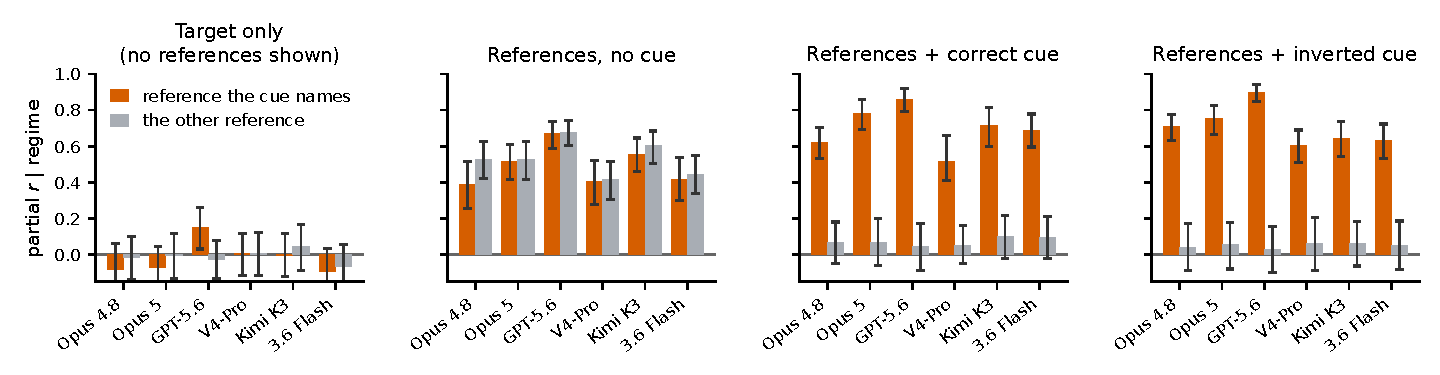
\includegraphics[width=\linewidth]{figures/exp2_reference_selection.pdf}
\caption{\textbf{The cue selects one of the two displayed references.} Partial
correlation between each deployment's forecast-implied City C slope and a
reference city's own fitted slope at $k=0$, controlling for the response regime
the City C sentence names; bars are 95\% episode-bootstrap intervals. Orange is
the reference that sentence points to, gray the other. With no reference cases
displayed neither loads; with both displayed and no cue they load equally, the
signature of pooling; the correct cue concentrates loading on the reference it
names; and an inverted cue moves that loading onto the reference it falsely names.
A prior attached to the words \emph{national} and \emph{local} predicts no
loading in any panel. Per-deployment values and the arbitrary-symbol version are in
Appendix~\ref{app:coin-city-reference-selection}.}
\label{fig:coin-city-reference-selection}
\end{figure}

\begin{center}
\begin{minipage}{\linewidth}
\centering
\captionof{table}{Partial correlation between the forecast-implied City C slope and
each reference city's fitted slope at $k=0$, controlling for the regime the City C
label names. ``Named'' is the reference the label points to, or the regime-matched
reference in the two arms without a label. Boldface marks named-reference intervals
excluding zero.}
\label{tab:coin-city-reference-selection}
\small
\setlength{\tabcolsep}{4pt}
% Generated by paper/generate_coin_city_reference_selection_tables.py from analysis/reference_selection_results.json; do not edit.
\begin{tabular}{l cc cc cc cc}
\toprule
& \multicolumn{2}{c}{Target only} & \multicolumn{2}{c}{ABC, no label}
& \multicolumn{2}{c}{ABC + correct} & \multicolumn{2}{c}{ABC + inverted} \\
\cmidrule(lr){2-3}\cmidrule(lr){4-5}\cmidrule(lr){6-7}\cmidrule(lr){8-9}
Model & Named & Other & Named & Other & Named & Other & Named & Other \\
\midrule
Claude Opus~4.8 & $-.08$ & $-.02$ & \textbf{$.39$} & $.53$ & \textbf{$.62$} & $.07$ & \textbf{$.71$} & $.04$ \\
GPT-5.6 & \textbf{$.15$} & $-.03$ & \textbf{$.67$} & $.68$ & \textbf{$.86$} & $.04$ & \textbf{$.90$} & $.03$ \\
DeepSeek V4-Pro & $.00$ & $.01$ & \textbf{$.40$} & $.42$ & \textbf{$.51$} & $.05$ & \textbf{$.61$} & $.06$ \\
Kimi K3 & $-.01$ & $.04$ & \textbf{$.55$} & $.60$ & \textbf{$.71$} & $.10$ & \textbf{$.64$} & $.06$ \\
Gemini 3.6 Flash & $-.09$ & $-.07$ & \textbf{$.42$} & $.44$ & \textbf{$.69$} & $.09$ & \textbf{$.63$} & $.05$ \\
Claude Opus~5 & $-.07$ & $-.00$ & \textbf{$.52$} & $.53$ & \textbf{$.78$} & $.07$ & \textbf{$.75$} & $.05$ \\
\bottomrule
\end{tabular}

\end{minipage}
\end{center}

The four arms make four different predictions and all four hold. With no reference
cases displayed at all, the target-only arm loads on neither reference: eleven of
its twelve intervals span zero. With both references displayed but no City C label,
every deployment loads on the two references almost equally, the pooling signature
of a model that cannot tell which reference applies. Adding the correct label
concentrates the loading on the named reference and removes it from the other,
every ``other'' interval spanning zero. Inverting the label moves the loading
wholesale onto the reference that the false cue names, leaving the truth-matched
reference near zero.

The forecast therefore tracks the particular reference city the label names,
including that city's sampling error, whether or not the label is correct. No
prior attached to the words \emph{national} and \emph{local} reproduces this. It
also explains why implied-slope correlations plateau near $.66$ rather than near
$.996$: faithful transfer of a noisy reference estimate is capped at that
reference's own $.656$ correlation with the truth. GPT-5.6 and Claude Opus~4.8
slightly exceed the cap at $k=0$, which is what blending a reference estimate with
a regime prior produces.

\paragraph{The estimator only detects an inefficiency.} The signal this analysis
reads is noise the forecast did not have to import. Each city draws its slope
independently, so a reference city's deviation from its regime mean is
uncorrelated with City C's: simulating the generator gives
$\operatorname{corr}(\widehat\beta^{\mathrm{ref}}-\mu,\;g_C-\mu)=-.0000$
(Section~\ref{app:coin-city-probe-ceilings}). Within a regime the reference's
fitted slope is therefore pure sampling error about a mean the regime already
supplies, and the response-recovery-optimal policy is to read the cue, ignore the
reference numbers, and predict the regime mean---which attains $\rho=.996$ against
the $.656$ a faithful transfer is capped at. A forecaster that did this would show
no loading on either reference and would be indistinguishable, under this
estimator, from the lexical-prior account the section argues against. The
estimator thus identifies reference selection only in forecasters that fail to
shrink, and has least power on those closest to the shrinking policy: the two
deployments above the transfer cap are the two with the highest slope
correlation, one of which also has the lowest $k=0$ forecast error of the six. We read a
positive loading as evidence for reference selection, and a null under this
estimator as uninformative rather than as evidence for a prior.

\begin{center}
\begin{minipage}{\linewidth}
\centering
\captionof{table}{The same partial correlation in the arbitrary-symbol arm at
$k=0$, where \texttt{KIV} and \texttt{ZOR} carry no stated direction and their
mapping reverses across episodes. The no-label columns repeat each model's pooling
control. Boldface marks symbol named-reference intervals excluding zero.}
\label{tab:coin-city-reference-selection-symbol}
\small
\setlength{\tabcolsep}{4pt}
% Generated by paper/generate_coin_city_reference_selection_tables.py from analysis/reference_selection_results.json; do not edit.
\begin{tabular}{l r cc cc}
\toprule
& & \multicolumn{2}{c}{ABC, no label} & \multicolumn{2}{c}{ABC + symbol} \\
\cmidrule(lr){3-4}\cmidrule(lr){5-6}
Model & $n$ & Named & Other & Named & Other \\
\midrule
Qwen3-4B & 250 & $.05$ & $-.09$ & $.00$ & $-.03$ \\
Qwen2.5-7B & 250 & $.11$ & $.15$ & \textbf{$.28$} & $.10$ \\
Qwen3-8B & 250 & $.12$ & $.06$ & $.09$ & $.11$ \\
Qwen2.5-14B & 250 & $.31$ & $.20$ & \textbf{$.32$} & $.03$ \\
Qwen3-14B & 250 & $.26$ & $.20$ & \textbf{$.46$} & $.06$ \\
Qwen3-32B & 250 & $.20$ & $.19$ & \textbf{$.40$} & $.03$ \\
Qwen2.5-32B & 250 & $.22$ & $.15$ & \textbf{$.38$} & $.02$ \\
Qwen2.5-72B & 250 & $.25$ & $.18$ & \textbf{$.53$} & $.04$ \\
Llama~3.1 8B & 249 & $-.02$ & $.07$ & $-.00$ & $-.08$ \\
Llama~3.1 70B & 250 & $.28$ & $.19$ & \textbf{$.54$} & $.00$ \\
DeepSeek V4-Pro & 250 & $.40$ & $.42$ & \textbf{$.51$} & $.07$ \\
Kimi K3 & 250 & $.55$ & $.60$ & \textbf{$.86$} & $.01$ \\
Claude Opus~4.8 & 250 & $.39$ & $.53$ & \textbf{$.71$} & $-.05$ \\
Claude Opus~5 & 250 & $.52$ & $.53$ & \textbf{$.83$} & $.02$ \\
GPT-5.6 Sol & 250 & $.67$ & $.68$ & \textbf{$.98$} & $.02$ \\
\bottomrule
\end{tabular}

\end{minipage}
\end{center}

Applying the estimator to the arbitrary-symbol arm removes the lexical account
entirely. Twelve of the fifteen released systems have a named-reference interval
excluding zero, and the three that do not---Qwen3-4B, Qwen3-8B and
Llama~3.1-8B---are exactly the three whose symbol-minus-no-context $\Delta\rho$
intervals span zero in Table~\ref{tab:coin-city-symbol-context}. The two
statistics are computed from different quantities and agree on all fifteen
systems.

\subsection{Linear-Probe Analysis of Cue-Conditioned Representations}
\label{app:coin-city-mechanistic-probe}

\subsubsection{Behavioral Screening Criteria}
We screen the same held-out prompts with Qwen3-8B, Qwen3-14B, dense Qwen3-32B, and
Qwen2.5-72B-Instruct. Each checkpoint received 16 test episodes crossed with
$k\in\{0,4\}$ and correct, absent, or inverted City C context (96 prompts), with
96/96 parseable forecasts.

\begin{center}
\begin{minipage}{\linewidth}
\centering
\captionof{table}{\textbf{Behavioral screening results for the linear-probe analysis.}
Entries are paired mean differences with 95\% episode-bootstrap intervals
($n=16$). Evidence is no-context $k=4$ minus $k=0$ aligned slope; selection is
correct minus absent context at $k=0$; reversal is inverted minus correct context
at $k=0$; forecast penalty is inverted minus correct poll MAE at $k=0$. Positive
evidence and selection, negative reversal, and a positive forecast penalty are
the predicted directions.}
\label{tab:coin-city-behavioral-gate}
\scriptsize
\setlength{\tabcolsep}{2.4pt}
\resizebox{\linewidth}{!}{% Generated by paper/generate_coin_city_mechanistic_comparison.py; do not edit.
\begin{tabular}{lcccc}
\toprule
Model & Evidence & Selection & Reversal & Forecast penalty \\
\midrule
Qwen3-8B & $+.119$ $[-.094,+.374]$ & $+.078$ $[-.012,+.219]$ & $-.140$ $[-.315,+.007]$ & $+.812$ $[-.063,+2.023]$ \\
Qwen3-14B & $+.394$ $[+.152,+.734]$ & $+.261$ $[+.134,+.400]$ & $-.380$ $[-.597,-.172]$ & $+1.662$ $[+.252,+3.155]$ \\
Qwen3-32B & $+.315$ $[+.017,+.646]$ & $+.234$ $[+.111,+.407]$ & $-.390$ $[-.554,-.221]$ & $+1.965$ $[+1.013,+3.083]$ \\
Qwen2.5-72B & $+.246$ $[+.001,+.529]$ & $+.096$ $[-.077,+.259]$ & $-.433$ $[-.674,-.220]$ & $+2.206$ $[+.957,+3.620]$ \\
\bottomrule
\end{tabular}
}
\end{minipage}
\end{center}

The 14B and 32B intervals exclude zero in all four predicted directions. For 72B,
the evidence, reversal, and forecast-penalty intervals exclude zero, while the
correct-versus-absent selection interval spans zero. All four 8B intervals span
zero. We use 32B for the dense Qwen3 scaling comparison and 72B for a
cross-generation comparison; neither is interpreted as another point on a
monotonic size curve. Qwen3-4B and Llama-3.1-8B use the identical task file,
held-out split, and model, layer, target, and endpoint selection rules.

\subsubsection{Activation and Probe Protocol}
We selected 64 episodes without replacement, balanced over which reference city
was strongly responsive and whether City C's latent regime was strong or weak.
Forty-eight episodes form a development set and 16 form a sealed test set. Each
episode is rendered at $k=0$ and $k=4$ under correct, absent, and inverted context,
giving 384 activation records. Within an episode-prefix pair the three prompts
have identical numeric content. The only intervention is the City C relationship
description.

For the final input token, we save the embedding output and every transformer-block
output. The resulting tensor dimensions are $[384,37,2560]$ for Qwen3-4B;
$[384,37,4096]$ for Qwen3-8B; $[384,33,4096]$ for Llama-3.1-8B;
$[384,41,5120]$ for Qwen3-14B; $[384,65,5120]$ for Qwen3-32B; and
$[384,81,8192]$ for Qwen2.5-72B-Instruct. We fit separate dual-ridge probes at
each layer and $k$, using only correct-context development episodes. Four
cell-balanced development folds select the ridge strength from
$\{10^{-4},3\!\times\!10^{-3},10^{-1},3,100\}$ and then select one reported
layer. The untouched test episodes are evaluated in all three context arms
($n=16$ per arm). A 10,000-repeat held-out label permutation test keeps the
development-selected layer, ridge strength, and fitted probe fixed. Thus neither
the test labels nor test-arm scores select the reported layer.

We probe three increasingly strict targets: the binary strong/weak regime; the
full realized slope $g_C$; and the within-regime residual
$g_C-.90$ for strong episodes or $g_C-.25$ for weak episodes. The first two are
recoverable from the displayed evidence and the third is not, by construction:
Section~\ref{app:coin-city-probe-ceilings} derives what a Bayes-optimal reader of
the same prompt could score on each, and the residual is included as a
specificity control rather than as a target a model could hit. Mean-pooled
embedding and final-layer states are additional pooling controls.

\begin{center}
\begin{minipage}{\linewidth}
\centering
\captionof{table}{\textbf{Six-model correct-context probe summary.}
Each entry gives $k=0/k=4$ on the 16 sealed episodes. Layers and ridge strengths
were selected on development episodes only. Residual $p$ is the one-sided
10,000-repeat held-out label-permutation value.}
\label{tab:coin-city-mechanistic-summary}
\small
\setlength{\tabcolsep}{3.0pt}
\resizebox{\linewidth}{!}{% Generated by paper/generate_coin_city_mechanistic_comparison.py; do not edit.
\begin{tabular}{lcccc}
\toprule
Model & Regime AUC & Full-slope $R^2$ & Residual-slope $R^2$ & Residual $p$ \\
\midrule
Qwen3-4B & 1.000/1.000 & .960/.885 & -.389/-.227 & .927/.614 \\
Qwen3-8B & .844/1.000 & .713/.653 & -.359/-.374 & .502/.735 \\
Llama-3.1-8B & 1.000/.984 & .913/.731 & -.126/-.207 & .380/.572 \\
Qwen3-14B & 1.000/.984 & .898/.627 & -.531/-.128 & .315/.450 \\
Qwen3-32B & 1.000/1.000 & .967/.811 & -.269/.003 & .477/.221 \\
Qwen2.5-72B & 1.000/1.000 & .975/.869 & -.451/-.053 & .675/.447 \\
\bottomrule
\end{tabular}
}
\end{minipage}
\end{center}

\begin{center}
\begin{minipage}{\linewidth}
\centering
\captionof{table}{\textbf{Held-out layer-wise open-weight probe.} AUC is reported
for the regime target and $R^2$ for both slope targets. Correct, none, and wrong
score the same development-selected probe against the true City C target under
the three context arms; wrong/cue instead scores the inverted arm against the
relationship named by its cue. $p$ is the one-sided held-out label-permutation
value on the correct-context test episodes.}
\label{tab:coin-city-mechanistic-probe}
\scriptsize
\setlength{\tabcolsep}{2.4pt}
\resizebox{\linewidth}{!}{% Generated by paper/generate_coin_city_mechanistic_comparison.py; do not edit.
\begin{tabular}{lllr rrrrrr}
\toprule
Model & $k$ & Target & Layer & Dev CV & Correct & None & Wrong/true & Wrong/cue & $p$ \\
\midrule
Qwen3-4B & 0 & Regime (AUC) & 1 & 1.000 & 1.000 & .562 & .000 & 1.000 & $<.001$ \\
 &  & Full slope ($R^2$) & 24 & .936 & .960 & -.517 & -2.614 & .956 & $<.001$ \\
 &  & Residual slope ($R^2$) & 15 & .054 & -.389 & -.296 & -.258 & -- & $.927$ \\
\cmidrule(lr){2-10}
 & 4 & Regime (AUC) & 19 & 1.000 & 1.000 & .609 & .094 & .906 & $<.001$ \\
 &  & Full slope ($R^2$) & 20 & .805 & .885 & -.065 & -1.147 & .492 & $<.001$ \\
 &  & Residual slope ($R^2$) & 14 & .004 & -.227 & .089 & -.183 & -- & $.614$ \\
\midrule
Qwen3-8B & 0 & Regime (AUC) & 19 & 1.000 & .844 & .453 & .078 & .922 & $.009$ \\
 &  & Full slope ($R^2$) & 23 & .870 & .713 & -.697 & -2.344 & .771 & $<.001$ \\
 &  & Residual slope ($R^2$) & 1 & .063 & -.359 & -.673 & -.378 & -- & $.502$ \\
\cmidrule(lr){2-10}
 & 4 & Regime (AUC) & 23 & .925 & 1.000 & .578 & .000 & 1.000 & $<.001$ \\
 &  & Full slope ($R^2$) & 23 & .462 & .653 & -.512 & -1.550 & .693 & $<.001$ \\
 &  & Residual slope ($R^2$) & 33 & .030 & -.374 & -1.003 & -.029 & -- & $.735$ \\
\midrule
Llama-3.1-8B & 0 & Regime (AUC) & 1 & 1.000 & 1.000 & .359 & .000 & 1.000 & $<.001$ \\
 &  & Full slope ($R^2$) & 1 & .907 & .913 & -18.953 & -2.629 & .972 & $<.001$ \\
 &  & Residual slope ($R^2$) & 12 & .018 & -.126 & -.458 & -.227 & -- & $.380$ \\
\cmidrule(lr){2-10}
 & 4 & Regime (AUC) & 1 & 1.000 & .984 & .438 & .000 & 1.000 & $<.001$ \\
 &  & Full slope ($R^2$) & 1 & .751 & .731 & -15.450 & -2.082 & .808 & $<.001$ \\
 &  & Residual slope ($R^2$) & 10 & .006 & -.207 & -.148 & -.150 & -- & $.572$ \\
\midrule
Qwen3-14B & 0 & Regime (AUC) & 2 & 1.000 & 1.000 & .422 & .000 & 1.000 & $<.001$ \\
 &  & Full slope ($R^2$) & 26 & .874 & .898 & -.522 & -2.423 & .943 & $<.001$ \\
 &  & Residual slope ($R^2$) & 34 & .159 & -.531 & -9.255 & -.096 & -- & $.315$ \\
\cmidrule(lr){2-10}
 & 4 & Regime (AUC) & 26 & .880 & .984 & .688 & .109 & .891 & $<.001$ \\
 &  & Full slope ($R^2$) & 26 & .408 & .627 & -.411 & -1.191 & .409 & $<.001$ \\
 &  & Residual slope ($R^2$) & 1 & -.013 & -.128 & -.605 & -.159 & -- & $.450$ \\
\midrule
Qwen3-32B & 0 & Regime (AUC) & 27 & 1.000 & 1.000 & .359 & .000 & 1.000 & $<.001$ \\
 &  & Full slope ($R^2$) & 47 & .930 & .967 & -.027 & -2.570 & .958 & $<.001$ \\
 &  & Residual slope ($R^2$) & 1 & .062 & -.269 & -.232 & -.259 & -- & $.477$ \\
\cmidrule(lr){2-10}
 & 4 & Regime (AUC) & 44 & 1.000 & 1.000 & .562 & .000 & 1.000 & $<.001$ \\
 &  & Full slope ($R^2$) & 47 & .797 & .811 & -.160 & -1.694 & .666 & $<.001$ \\
 &  & Residual slope ($R^2$) & 1 & .043 & .003 & .062 & -.000 & -- & $.221$ \\
\midrule
Qwen2.5-72B & 0 & Regime (AUC) & 53 & 1.000 & 1.000 & .469 & .000 & 1.000 & $<.001$ \\
 &  & Full slope ($R^2$) & 58 & .955 & .975 & -1.050 & -2.958 & .969 & $<.001$ \\
 &  & Residual slope ($R^2$) & 32 & .061 & -.451 & -1.192 & -.401 & -- & $.675$ \\
\cmidrule(lr){2-10}
 & 4 & Regime (AUC) & 58 & .995 & 1.000 & .922 & .062 & .938 & $<.001$ \\
 &  & Full slope ($R^2$) & 58 & .678 & .869 & -.468 & -1.072 & .493 & $<.001$ \\
 &  & Residual slope ($R^2$) & 1 & -.017 & -.053 & -.063 & -.053 & -- & $.447$ \\
\bottomrule
\end{tabular}
}
\end{minipage}
\end{center}

\begin{figure}[ht]
  \centering
  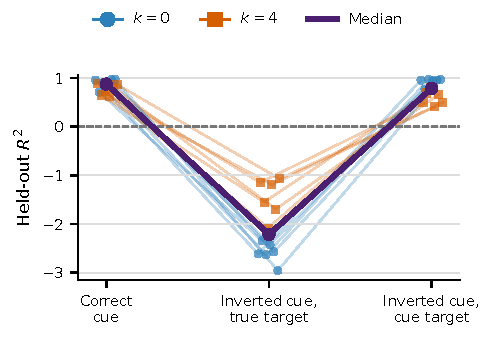
\includegraphics[width=.62\linewidth]{figures/exp2_qwen3_mechanistic_main.pdf}
  \caption{\textbf{Semantic-arm slope decoding follows cue assignment.}
  Each line is a sealed model--$k$ cell across the six open checkpoints of the
  16-episode roster; purple is the median. Probes are fit on correct-context
  development episodes. Under inversion, held-out $R^2$ collapses against the true
  slope and recovers against the cue-assigned slope. The input-embedding control
  below shows this signal is available before any computation, which is why the
  arbitrary-label replication rather than this figure carries the
  representational claim.}
  \label{fig:coin-city-mechanistic-main}
\end{figure}

\begin{figure}[ht]
  \centering
  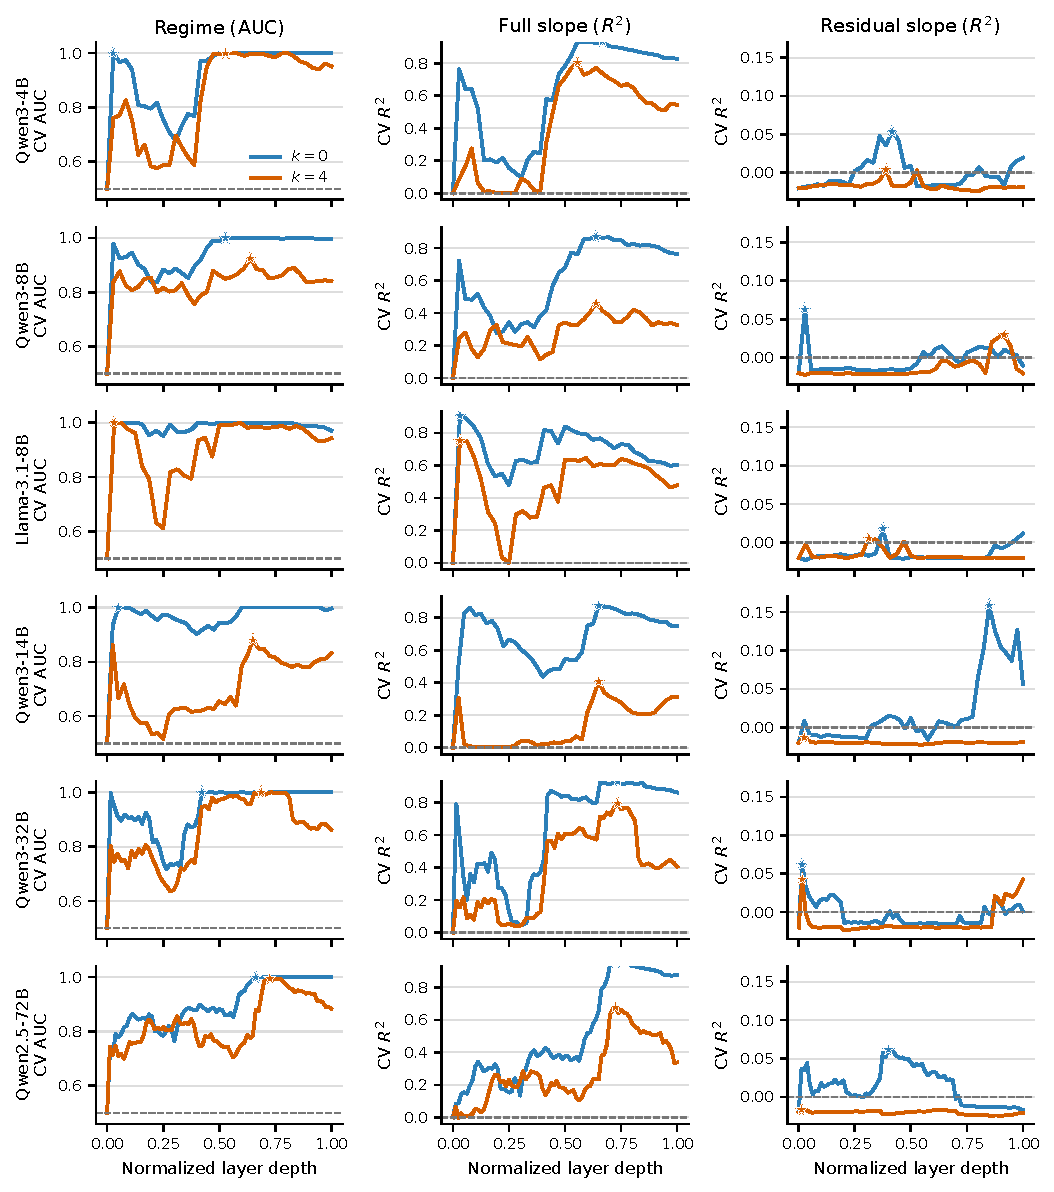
\includegraphics[width=\linewidth]{figures/exp2_qwen3_mechanistic_probe.pdf}
  \caption{\textbf{Development layer trajectories for the six-model probe.}
  Curves show four-fold development CV rather than test performance; stars mark
  the development-selected layer. Layer depth is normalized
  because the checkpoints have 32--80 transformer blocks. The regime and
  full-slope signals are broad, whereas residual-slope CV is weak and does not
  survive held-out evaluation.}
  \label{fig:coin-city-mechanistic-probe}
\end{figure}

\subsubsection{Regime and Full-Slope Decodability}
Across the six checkpoints and two evidence depths, correct-context regime AUC
is $.844$--$1.000$ and full-slope $R^2$ is $.627$--$.975$
(Table~\ref{tab:coin-city-mechanistic-summary}). This information is not a
context-invariant encoding of the true coefficient: removing the City C
description drives selected-layer full-slope $R^2$ below zero in all 12
model--$k$ cells. Under inversion, true-target regime AUC falls to
$.000$--$.109$ while cue-target AUC is $.891$--$1.000$; the full-slope probe
likewise fits the cue-assigned relationship better than the true one. The Llama
replication shows that this pattern is not specific to the Qwen checkpoints.
Across both model families, the linearly available signal therefore tracks the
response family that context assigns to City C.

\subsubsection{What Each Probe Target Can Be Scored Against}
\label{app:coin-city-probe-ceilings}

A probe is scored against a latent generator quantity, so a null is only a fact
about a model if the displayed evidence determines that quantity. We therefore
derive, for each target and evidence depth, the score a Bayes-optimal reader of
the same prompt would obtain. This is an analytic property of
Equation~\ref{eq:coin-city-dgp} and its row construction, computed in closed form
and re-derived by simulating the generator's own row logic; the two agree to
within $.005$ and no model output enters; the derivation is
\path{exp2_v2/biased_news/analysis/compute_bayes_ceilings.py}.
Table~\ref{tab:coin-city-probe-ceilings} gives the ceilings. The same module
reports forecast-MAE floors: $2.28$ poll points at $k=0$ with no cue, $0.17$ for
an oracle told the regime means, and $1.78$ for a reader who must instead estimate
the named regime's slope from its four displayed rows.

The same simulation records one quantity the reference-selection analysis of
Section~\ref{app:coin-city-reference-selection} depends on. Cities draw their
slopes independently, so a reference city's deviation from its regime mean
carries no information about City C's:
$\operatorname{corr}(\widehat\beta^{\mathrm{ref}}-\mu,\;g_C-\mu)=-.0000$ over
400,000 simulated episodes, against a reference-fit standard deviation of $.318$
within regime. That is why a loading on the reference's own sampling error
identifies reference selection, and equally why a forecaster that shrank
optimally would show none.

\begin{center}
\begin{minipage}{\linewidth}
\centering
\captionof{table}{Maximum score a Bayes-optimal reader of the same prompt can
obtain on each probe target, under the frozen data-generating process. The regime
and the full slope are recoverable; the within-regime residual is not, because it
is generated with standard deviation $.03$ while a through-origin fit to City C's
displayed rows carries a standard deviation of $.318$. At $k=0$ City C displays no
rows at all and the residual ceiling is exactly zero.}
\label{tab:coin-city-probe-ceilings}
\small
% Generated by exp2_v2/biased_news/analysis/compute_bayes_ceilings.py; do not edit.
\begin{tabular}{llcc}
\toprule
\textbf{Probe target} & & $k=0$ & $k=4$ \\
\midrule
Regime, correct semantic cue & AUC & 1.000 & 1.000 \\
Regime, arbitrary label & AUC & 0.979 & --- \\
Full slope $g_C$ & $R^2$ & 0.992 & 0.992 \\
Residual slope $g_C-\mu$ & $R^2$ & 0.000 & 0.009 \\
\bottomrule
\end{tabular}

\end{minipage}
\end{center}

\subsubsection{Specificity: Within-Regime Residuals}
The residual target is the specificity control, and it behaves as a target with
no available signal should. The 12 correct-context residual-slope $R^2$ values
range from $-.531$ to $.003$, none of their permutation tests rejects the null
($p=.221$--$.927$), and 33 of 36 arm-level residual scores are nonpositive.
Against a ceiling of $.000$ at $k=0$ and $.009$ at $k=4$, that is the result the
design permits: no reader of these prompts, and no representation computed from
them, could score materially above zero. We therefore read the residual null as
evidence that the probe does not manufacture structure where none is available,
and not as a limit on what these checkpoints encode. A probe that returned a
positive residual score here would be the finding, and it would be a warning
about the probe.

The two recoverable targets do carry information, and the input-embedding control
is what bounds their interpretation. Mean-pooled input embeddings for every Qwen
checkpoint already give perfect regime AUC and full-slope $R^2=.988$--$.993$ under
correct context---at the $.992$ ceiling---because the explicit description names a
regime and the regime means account for essentially all slope variance. Llama
input embeddings likewise give perfect regime AUC and full-slope $R^2=.756/.827$.
The layer-wise semantic result is therefore evidence that the cue-selected
response family is linearly represented, and reaches nothing further about the
continuous $g_C$: the part of $g_C$ beyond the family is not in the prompt to
begin with. The original behavioral inversion screen connects this representation
to output sensitivity in the three larger screened checkpoints: inverted context
raises $k=0$ forecast MAE by $1.66$, $1.96$, and $2.21$ points for 14B, 32B, and
72B, respectively.

\subsubsection{Power-Matched and Cross-Model Arbitrary-Symbol Replication}
\label{app:coin-city-probe-power}

The six-checkpoint roster above seals 16 test episodes per arm. Its exact
label-permutation null spans ROC AUC $[.203,.797]$, so it can separate a score
from chance only above about $.75$. That resolution suffices for the semantic arm,
whose scores sit at ceiling, but it cannot evaluate a weaker signal at all. We
therefore evaluate Qwen3-14B at the design's balanced maximum---248
episodes, 160 development and 88 sealed test, 1,488 activation records---once with
the semantic cue and once with the episode-randomized \texttt{KIV}/\texttt{ZOR}
labels. Anchor, targets, fold structure, ridge grid, layer-selection rule, pooling
controls and the 10,000-repeat held-out permutation test are unchanged; only the
number of episodes differs. The 88-episode null reaches AUC $.603$. The enlarged
development set is disjoint from every episode used by the 16-episode analysis,
providing an independent estimate rather than a re-slice.

\begin{center}
\begin{minipage}{\linewidth}
\centering
\captionof{table}{\textbf{Power-matched Qwen3-14B probe, 88 sealed episodes per
arm.} Correct, none and wrong score the development-selected probe against the true
City C target under the three cue arms; wrong/cue scores the inverted arm against
the relationship its cue names. ``Layer'' is the development-selected block of 40
and ``Embed.'' is the mean-pooled input-embedding control under correct context.
$p$ is the one-sided held-out label-permutation value.}
\label{tab:coin-city-probe-power}
\scriptsize
\setlength{\tabcolsep}{3.2pt}
\resizebox{\linewidth}{!}{% Generated by paper/generate_coin_city_probe_power_table.py; do not edit.
\begin{tabular}{l l rrrr r r r r}
\toprule
Run & Target & Correct & None & Wrong & Wrong/cue & Layer & Embed. & $p$ & Behav. $\Delta\rho$ \\
\midrule
Qwen3-14B, semantic & $k{=}0$ regime AUC & $1.000$ & $.429$ & $.000$ & $1.000$ & 1 & $1.000$ & $<$.001 & --- \\
 & $k{=}4$ regime AUC & $1.000$ & $.560$ & $.000$ & $1.000$ & 1 & $1.000$ & $<$.001 &  \\
 & $k{=}0$ slope $R^2$ & $.942$ & $-.300$ & $-2.806$ & $.961$ & 27 & $.989$ & $<$.001 &  \\
 & $k{=}4$ slope $R^2$ & $.910$ & $-24.039$ & $-2.387$ & $.906$ & 1 & $.989$ & $<$.001 &  \\
\midrule
Qwen3-14B, symbol & $k{=}0$ regime AUC & $.678$ & $.467$ & $.321$ & $.679$ & 26 & $.555$ & $.0016$ & \textbf{$.398$} \\
 & $k{=}4$ regime AUC & $.713$ & $.689$ & $.747$ & $.253$ & 40 & $.582$ & $<$.001 &  \\
 & $k{=}0$ slope $R^2$ & $.016$ & $-.094$ & $-.130$ & $.065$ & 26 & $.003$ & $.1162$ &  \\
 & $k{=}4$ slope $R^2$ & $.030$ & $-.237$ & $.126$ & $-.855$ & 40 & $-.032$ & $<$.001 &  \\
\midrule
Qwen3-8B, symbol & $k{=}0$ regime AUC & $.566$ & $.535$ & $.567$ & $.433$ & 10 & $.534$ & $.1471$ & $.023$ \\
 & $k{=}4$ regime AUC & $.610$ & $.545$ & $.593$ & $.407$ & 19 & $.621$ & $.0401$ &  \\
 & $k{=}0$ slope $R^2$ & $-.001$ & $.005$ & $.004$ & $-.007$ & 25 & $.003$ & $.4883$ &  \\
 & $k{=}4$ slope $R^2$ & $-.151$ & $-.219$ & $-.188$ & $-.504$ & 20 & $-.018$ & $.0314$ &  \\
\midrule
Qwen3-4B, symbol & $k{=}0$ regime AUC & $.520$ & $.419$ & $.329$ & $.671$ & 23 & $.498$ & $.3756$ & $.095$ \\
 & $k{=}4$ regime AUC & $.685$ & $.689$ & $.637$ & $.363$ & 22 & $.585$ & $.0017$ &  \\
 & $k{=}0$ slope $R^2$ & $-.009$ & $-.065$ & $-.079$ & $.023$ & 23 & $.004$ & $.2899$ &  \\
 & $k{=}4$ slope $R^2$ & $-.021$ & $-.265$ & $-.031$ & $-.687$ & 23 & $.004$ & $.0014$ &  \\
\midrule
Qwen2.5-32B, symbol & $k{=}0$ regime AUC & $.778$ & $.571$ & $.200$ & $.800$ & 50 & $.550$ & $<$.001 & \textbf{$.372$} \\
 & $k{=}4$ regime AUC & $.797$ & $.831$ & $.662$ & $.338$ & 46 & $.589$ & $<$.001 &  \\
 & $k{=}0$ slope $R^2$ & $.217$ & $-.256$ & $-1.033$ & $.254$ & 50 & $.004$ & $<$.001 &  \\
 & $k{=}4$ slope $R^2$ & $.263$ & $-.563$ & $-.044$ & $-.774$ & 46 & $-.029$ & $<$.001 &  \\
\midrule
Qwen2.5-72B, symbol & $k{=}0$ regime AUC & $.662$ & $.492$ & $.210$ & $.790$ & 63 & $.556$ & $.0026$ & \textbf{$.381$} \\
 & $k{=}4$ regime AUC & $.793$ & $.745$ & $.651$ & $.349$ & 61 & $.575$ & $<$.001 &  \\
 & $k{=}0$ slope $R^2$ & $-.005$ & $-.490$ & $-1.034$ & $.187$ & 62 & $.004$ & $.0072$ &  \\
 & $k{=}4$ slope $R^2$ & $.222$ & $-.624$ & $-.129$ & $-.870$ & 61 & $-.047$ & $<$.001 &  \\
\midrule
Llama~3.1-8B, symbol & $k{=}0$ regime AUC & $.423$ & $.447$ & $.452$ & $.548$ & 11 & $.539$ & $.8925$ & $.045$ \\
 & $k{=}4$ regime AUC & $.543$ & $.604$ & $.549$ & $.451$ & 31 & $.604$ & $.2470$ &  \\
 & $k{=}0$ slope $R^2$ & $-.097$ & $-.089$ & $-.086$ & $-.001$ & 11 & $.003$ & $.8607$ &  \\
 & $k{=}4$ slope $R^2$ & $-.275$ & $-.091$ & $-.156$ & $-.358$ & 31 & $.009$ & $.4529$ &  \\
\midrule
Llama~3.1-70B, symbol & $k{=}0$ regime AUC & $.728$ & $.468$ & $.292$ & $.708$ & 75 & $.495$ & $<$.001 & \textbf{$.424$} \\
 & $k{=}4$ regime AUC & $.810$ & $.740$ & $.721$ & $.279$ & 42 & $.606$ & $<$.001 &  \\
 & $k{=}0$ slope $R^2$ & $.076$ & $-8.200$ & $-.961$ & $.082$ & 75 & $.003$ & $<$.001 &  \\
 & $k{=}4$ slope $R^2$ & $.222$ & $-3.224$ & $.087$ & $-1.007$ & 55 & $.007$ & $<$.001 &  \\
\bottomrule
\end{tabular}
}
\end{minipage}
\end{center}

The two arms separate sharply, and the input-embedding control is what separates
them. Under the semantic cue the development-selected layer is the first
transformer block for three of the four conditions, and mean-pooled input
embeddings alone already reach regime AUC $1.000$ and full-slope $R^2=.989$: the
decodable quantity is the cue token itself. Under arbitrary labels the same control
collapses to AUC $.555$ and $R^2=.003$, the selected layers move to blocks 26 and
40 of 40, and held-out regime AUC is $.678$ at $k=0$ ($p=.0016$) and $.713$ at
$k=4$ ($p<.001$). The induced label-to-regime mapping is therefore linearly
represented, but only after computation, far more weakly than a regime the model
was told outright, and below the $.979$ AUC a Bayes-optimal reader of the same two
reference cities could reach. Unlike the residual target, the full slope is
recoverable here---its ceiling is $.992$---so its symbol-arm score of $R^2=.016$ at
$k=0$, which does not reject its null, is a genuine gap rather than a property of
the design.

Representation and behavior agree closely once the cue must be induced. On the same
88 sealed episodes the model's own forecasts give regime AUC $.702$, $.518$ and
$.331$ under correct, absent and inverted labels, against probe AUCs of $.678$,
$.467$ and $.321$; inversion raises $k=0$ poll MAE from $2.49$ to $4.28$. With four
City C cases the inverted-arm representation reverses: true-target regime AUC rises
from $.321$ to $.747$, and the full-slope probe fits the cue-named relationship at
$R^2=-.855$ while fitting the true one at $+.126$. Direct target evidence overrides
the induced label in the representation as it does in the forecast.

Six further checkpoints received the identical symbol protocol at the same 88
sealed episodes: Qwen2.5-32B and Qwen2.5-72B, which change model generation;
Qwen3-8B and Qwen3-4B, which hold family, tokenizer and architecture fixed and
change only scale; and Llama~3.1-8B and Llama~3.1-70B, which do the same within a
second vendor and architecture. Held-out regime AUC at $k=0$ is $.778$ for
Qwen2.5-32B ($p<.001$, selected layer 50 of 64), $.728$ for Llama~3.1-70B
($p<.001$, layer 75 of 81), $.662$ for Qwen2.5-72B ($p=.003$, layer 63 of 80),
$.566$ for Qwen3-8B ($p=.15$), $.520$ for Qwen3-4B ($p=.38$) and $.423$ for
Llama~3.1-8B ($p=.89$). No null checkpoint rejects in any $k=0$
condition---regime, slope or residual slope. Mean-pooled input embeddings stay
between $.495$ and $.556$ in every symbol run, so no symbol arm carries the
mapping before computation.

Decodability tracks behavioral recovery across all seven checkpoints, four
positive and three null. The four whose forecasts recover the mapping are the four
in which it decodes (Llama~3.1-70B, $\Delta\rho=.424$; Qwen3-14B, $.398$;
Qwen2.5-72B, $.381$; Qwen2.5-32B, $.372$), and the three whose forecasts do not
are the three in which it does not (Qwen3-4B, $.095$; Llama~3.1-8B, $.045$;
Qwen3-8B, $.023$; all three intervals spanning zero). The Llama~3.1
contrast carries the weight, because it holds family, tokenizer and architecture
fixed, varies only scale, and is the one within-family contrast whose behavioral
classification survives the harder generator population of
Section~\ref{app:coin-city-robustness}: 8B is null on both populations and 70B
positive on both, while the probe runs $.423$ to $.728$ across them. Because the
null and the positive share an architecture and a tokenizer, the split is not an
artifact of either.

The Qwen3 sequence---$.520$, $.566$, $.678$ from 4B to 14B---is consistent with
this but does not add independent weight, because the population that would test
it is the one on which its behavioral boundary moves. That movement is smaller
than the $\Delta\rho$ column alone suggests. Symbol-arm regime accuracy orders the
four Qwen3 checkpoints identically in both populations, $.512$, $.516$, $.660$,
$.656$ originally against $.528$, $.554$, $.589$, $.606$ on the harder one: no
pair reverses, and what changes is that the harder population compresses every
score toward chance, so a threshold that fell in a clear gap now falls inside a
compressed continuum. The $\Delta\rho$ contrast then subtracts a no-context
baseline whose standard error is about $.064$, and baselines of $-.036$ for
Qwen3-8B and $+.025$ for Qwen3-14B are enough to put one interval above zero and
the other $.004$ below it, with the two intervals overlapping by $78\%$. We
therefore read the harder population as showing that the ordering replicates while
the significance threshold is not locatable to a checkpoint, rather than as a
reversal. Section~\ref{app:coin-city-robustness} should be read alongside the
seven-for-seven agreement, which is evidence that the probe reads what the
forecasts express on the episodes both were measured on and not evidence for a
scale law. The positives span three model generations and two
vendors, and every positive shows the same shape: the decoded regime follows the
cue at $k=0$ and the truth at $k=4$.
Qwen3-4B and Qwen3-8B do reject at $k=4$ ($.685$, $p=.002$ and $.610$, $p=.04$),
which is expected rather than contrary: at $k=4$ the displayed target cases
exhibit the regime whatever the label says, and the mean-pooled input embeddings
rise to $.585$ and $.621$ accordingly, in Qwen3-8B's case above the probe itself.
The induction claim is a $k=0$ claim throughout. The sealed test is 88 episodes
per model, well above the 16 the roster began with but not a large sample, and the
permutation nulls are computed rather than assumed.

At 16 episodes, the same arbitrary-symbol procedure returns $k=0$ regime AUC
$.312$ with $p=.90$. Its $[.203,.797]$ null is too broad to resolve a signal of
the magnitude observed at 88 episodes.

\subsubsection{Causal Test: Patching the City C Label Representation}
\label{app:coin-city-causal-patch}

Decodability is not mediation. To test whether the representation the probe reads
is the one the forecast uses, we intervene on it directly. Under arbitrary labels, an episode's correct and swapped prompts are
positionally aligned through the City C label and differ at exactly two label-token
positions.
We replace the residual stream at those two positions with the states the opposite
arm produces, in both directions, and regenerate the forecast greedily. The
endpoint is the episode-level mean of the regime-aligned correct-into-swapped
shift and the sign-reversed swapped-into-correct shift, tested one-sided against
an episode sign-flip null.

The analysis uses three patch sites and two controls. The primary site is a
three-layer window centred on the development-selected relational layer;
patching at the embedding output only, and at every causally effective layer, are
the comparison sites; the unpatched arm and a self-patch that writes each state
back over itself are the controls. Layer, window and ridge were selected on
development episodes with the sealed test unread.

\begin{center}
\begin{minipage}{\linewidth}
\centering
\captionof{table}{\textbf{Causal effect of patching the two City C symbol
subtokens, Qwen3-14B.} Shift is the regime-aligned symmetric patch mean; positive
means the forecast moved toward the relationship the donor label names. The
16- and 88-episode analyses select their windows independently on
their own development sets. The null interval is the 88-episode sign-flip null.}
\label{tab:coin-city-causal-patch}
\small
\setlength{\tabcolsep}{4pt}
\resizebox{\linewidth}{!}{% Generated by paper/generate_coin_city_causal_patch_table.py; do not edit.
\begin{tabular}{l c rrr rrr c}
\toprule
& & \multicolumn{3}{c}{16 sealed, window 33--35} & \multicolumn{3}{c}{88 sealed, window 19--21} & \\
\cmidrule(lr){3-5}\cmidrule(lr){6-8}
Patch site & $k$ & Shift & $p$ & $n$ & Shift & $p$ & $n$ & Null 95\% \\
\midrule
Selected window & $k{=}0$ & $-.033$ & $.75$ & 14 & $.333$ & $<$.0001 & 82 & $[-.177,.178]$ \\
 & $k{=}4$ & $-.007$ & $.75$ & 15 & $-.035$ & $.8256$ & 87 & $[-.073,.073]$ \\
\midrule
Embedding only & $k{=}0$ & $.236$ & $.15$ & 14 & $.319$ & $.0002$ & 84 & $[-.182,.182]$ \\
 & $k{=}4$ & $.115$ & $.23$ & 15 & $-.017$ & $.6419$ & 87 & $[-.087,.087]$ \\
\midrule
All layers & $k{=}0$ & $.236$ & $.15$ & 14 & $.319$ & $.0002$ & 84 & $[-.182,.182]$ \\
 & $k{=}4$ & $.115$ & $.23$ & 15 & $-.017$ & $.6419$ & 87 & $[-.087,.087]$ \\
\bottomrule
\end{tabular}
}
\end{minipage}
\end{center}

At $k=0$ the intervention moves the forecast: patching the selected window shifts
the regime-aligned prediction by $.333$ against a null interval of
$[-.177,.178]$ ($p<.0001$, 82 complete episodes), and patching the embedding
alone gives $.319$. All eight stability checks pass, including $347/347$ exact
self-patch matches.

Two readings of the table matter more than the significance. First, the
embedding-only and all-layer rows are identical, and necessarily so: the two
prefixes differ only at the patched label positions, so overwriting their embeddings
and letting the model recompute reproduces what overwriting every later state does. They are one intervention reported at two depths, not two
converging results. What distinguishes the mid-window row is that it reaches the
same magnitude while touching only three layers late in the network.

Second, the effect is confined to $k=0$. With four City C cases every patch site
returns a null ($p=.83$ and $p=.64$), so the induced label no longer controls the
forecast once direct target evidence is available. That is the revision claim of
Section~\ref{app:coin-city-results} in causal form, and it matches the
representational result: at $k=4$ the inverted-arm probe recovers the true regime
rather than the cue-assigned one.

At 16 episodes, the primary patch estimate is $-.033$ at $p=.75$ and the sign-flip
null spans $[-.387,.387]$. Its 64-episode development set selects layers
$33$--$35$, whereas the 160-episode development set selects $19$--$21$ at a
higher cross-validation score ($.903$ against $.806$).

\paragraph{Permutation implementation.} The test enumerates all $2^{n}$ sign
assignments for 16 episodes; exhaustive enumeration is infeasible for 88
($2^{88}\approx3\times10^{26}$). Enumeration is retained for $n\le20$; above it
the same null is sampled with $200{,}000$ draws under a fixed seed, giving a
Monte Carlo standard error of $.0005$ at $p=.05$. The estimand, endpoint, and
direction are identical under both implementations.

\paragraph{Scope.} This is one checkpoint under arbitrary labels. It shows that
the label representation Qwen3-14B computes is causally responsible for its
zero-shot regime assignment, and that direct evidence displaces it. It does not
establish the same for the hosted deployments, the semantic cue, or other
architectures.

\subsubsection{Reproducibility and Scope}
The checkpoints are pinned to commits
\texttt{cdbee75f17c01a7cc42f958dc650907174af0554} (Qwen3-4B),
\texttt{b968826d9c46dd6066d109eabc6255188de91218} (Qwen3-8B),
\texttt{0e9e39f249a16976918f6564b8830bc894c89659} (Llama-3.1-8B),
\texttt{40c069824f4251a91eefaf281ebe4c544efd3e18} (Qwen3-14B),
\texttt{9216db5781bf21249d130ec9da846c4624c16137} (Qwen3-32B), and
\texttt{495f39366efef23836d0cfae4fbe635880d2be31} (Qwen2.5-72B).
The activation hashes are
\texttt{e1913859\allowbreak{}63d639aa\allowbreak{}5b8574a9\allowbreak{}abbeb91b\allowbreak{}3519aed9\allowbreak{}34ac491f\allowbreak{}86365563\allowbreak{}1b26dbbc}
(Qwen3-4B) and
\texttt{7f65aeec\allowbreak{}7a91e404\allowbreak{}cc600686\allowbreak{}18fedf25\allowbreak{}c679abde\allowbreak{}5d48c2b8\allowbreak{}477f7366\allowbreak{}70fbc54f}
(Llama-3.1-8B); all six hashes and tensor dimensions are enforced by the
fail-closed generator. Frozen tasks, activation tensors, extraction manifests,
generated behavior, selected predictions, complete layer curves, and probe
results are under
\path{exp2_v2/biased_news/data/coin_city_stable_relationship_claude_n250_v4/mechanistic_probe/}.
The analysis and asset generator are
\path{exp2_v2/biased_news/mechanistic_probe/analyze_probe.py} and
\path{paper/generate_coin_city_mechanistic_comparison.py}. The causal run is
\path{mechanistic_probe/qwen3_14b_symbol_relational_v2/}, frozen by
\path{freeze_symbol_relational_protocol.py} and executed by
\path{extract_symbol_label_states.py}, \path{patch_symbol_label_activations.py}
and \path{analyze_symbol_relational_probe.py}; every count in that pipeline is
derived from the frozen task manifest and checked by
\path{tests/test_symbol_relational_scaling.py}.
\path{paper/generate_coin_city_causal_patch_table.py} fails closed on the run's
study name, sealed-test size and stability gate. The power-matched runs are
\path{mechanistic_probe/qwen3_14b_probe_v2/},
\path{mechanistic_probe/qwen3_14b_symbol_probe_v2/},
\path{mechanistic_probe/qwen3_8b_symbol_probe_v2/},
\path{mechanistic_probe/qwen3_4b_symbol_probe_v2/},
\path{mechanistic_probe/llama3_1_70b_symbol_probe_v2/},
\path{mechanistic_probe/qwen2_5_72b_symbol_probe_v2/},
\path{mechanistic_probe/qwen2_5_32b_symbol_probe_v2/} (checkpoint
\texttt{5ede1c97bbab6ce5cda5812749b4c0bdf79b18dd}) and
\path{mechanistic_probe/llama3_1_8b_symbol_probe_v2/} (checkpoint
\texttt{0e9e39f249a16976918f6564b8830bc894c89659}), built by
\path{exp2_v2/biased_news/mechanistic_probe/build_probe_tasks.py} and
\path{build_arbitrary_symbol_probe_tasks.py} with 62 and 31 episodes per factorial
cell; \path{paper/generate_coin_city_probe_power_table.py} regenerates their table
and validates the sealed-test size and task hash. Each run's
activation tensor is regenerable from its frozen task file and pinned checkpoint;
the extraction manifests record the tensor hashes rather than the tensors.
Cross-vendor probe evidence here is the Llama~3.1-8B null rather than a
positive. The diagnostic covers six checkpoints spanning Qwen and Llama at 16 sealed episodes per arm, plus
the matched 88-episode semantic and arbitrary-symbol Qwen3-14B pair. For the semantic
cue it is correlational and does not establish that the decoded direction
mediates the forecast; under arbitrary labels
Section~\ref{app:coin-city-causal-patch} provides a causal intervention for one
checkpoint. Both complement the paired behavioral interventions above.


\subsection{Robustness Across Generator Populations and Deployments}
\label{app:coin-city-robustness}

\subsubsection{Generator-population robustness}
Fresh seeds 940000--940249 target strong/weak means of \(.75/.40\)
with slope SD \(.10\), jointly narrowing the regime gap and widening
within-regime dispersion. The realized target slopes are
\(.752\pm.100\) and \(.404\pm.105\). Draws were neither truncated nor reordered:
two reference pairs reverse their nominal latent ordering and remain in the
analysis. Case noise, factorial balance, prompts, prefix set, local checkpoint
settings, and episode-randomized symbol mapping are unchanged.

All ten open checkpoints were run on the three matched arms, producing 37,500
response records; 37,355 contain a numeric forecast, and unresolved formats remain
missing. Table~\ref{tab:coin-city-generator-robustness} compares the
\(k=0\) symbol-minus-no-context contrast across generator populations. Bold
intervals exclude zero; negative \(\Delta\)MAE would favor symbol context.
Because this population changes separation and dispersion together, it tests the
joint perturbation rather than identifying either parameter's effect separately.

\begin{center}
\begin{minipage}{\linewidth}
\centering
\captionof{table}{Arbitrary-symbol recovery on the original and harder generator
populations. Intervals are 95\% episode-bootstrap intervals with 5,000 draws;
\(n\) is the harder-population complete-case count.}
\label{tab:coin-city-generator-robustness}
\scriptsize
\setlength{\tabcolsep}{2.5pt}
\resizebox{\linewidth}{!}{% Generated by paper/generate_coin_city_robustness_tables.py; do not edit.
\begin{tabular}{lrcccc}
\toprule
Model & $n$ & Original $\Delta\rho$ [95\% CI] & Harder $\Delta\rho$ [95\% CI] & Symbol acc. & Harder $\Delta$MAE [95\% CI] \\
\midrule
Qwen3-4B & 250 & $+.095$ $[-.060,.230]$ & $+.050$ $[-.079,.197]$ & .528 & $+.052$ $[-.056,.161]$ \\
Qwen3-8B & 249 & $+.023$ $[-.128,.171]$ & \textbf{$+.231$ $[.074,.370]$} & .554 & $-.113$ $[-.269,.036]$ \\
Qwen3-14B & 246 & \textbf{$+.398$ $[.253,.541]$} & $+.155$ $[-.004,.303]$ & .589 & \textbf{$+.361$ $[.076,.644]$} \\
Qwen3-32B & 249 & \textbf{$+.302$ $[.177,.433]$} & \textbf{$+.193$ $[.063,.325]$} & .606 & \textbf{$+.848$ $[.539,1.168]$} \\
Qwen2.5-7B & 250 & \textbf{$+.264$ $[.112,.406]$} & \textbf{$+.149$ $[.009,.279]$} & .540 & $+.303$ $[.000,.627]$ \\
Qwen2.5-14B & 250 & \textbf{$+.236$ $[.107,.356]$} & \textbf{$+.133$ $[.005,.254]$} & .584 & \textbf{$+.365$ $[.115,.609]$} \\
Qwen2.5-32B & 250 & \textbf{$+.372$ $[.226,.502]$} & \textbf{$+.247$ $[.109,.383]$} & .616 & \textbf{$+.882$ $[.590,1.186]$} \\
Qwen2.5-72B & 250 & \textbf{$+.381$ $[.250,.508]$} & \textbf{$+.336$ $[.204,.463]$} & .604 & \textbf{$+1.012$ $[.717,1.316]$} \\
Llama~3.1-8B & 229 & $+.045$ $[-.123,.250]$ & $-.077$ $[-.216,.079]$ & .524 & \textbf{$+.597$ $[.229,.952]$} \\
Llama~3.1-70B & 249 & \textbf{$+.424$ $[.314,.543]$} & \textbf{$+.242$ $[.119,.369]$} & .558 & \textbf{$+.856$ $[.465,1.242]$} \\
\bottomrule
\end{tabular}
}
\end{minipage}
\end{center}

Which Qwen3 checkpoints clear significance changes, but their ordering does not.
Qwen3-8B moves from an original null to \(\Delta\rho=.231\) \([.074,.370]\) while
Qwen3-14B falls to \(.155\) \([-.004,.303]\); Qwen3-4B remains null and Qwen3-32B
remains positive. Regime accuracy in the symbol arm, which subtracts no baseline,
orders the four identically in both populations---\(.512\), \(.516\), \(.660\),
\(.656\) originally against \(.528\), \(.554\), \(.589\), \(.606\) here---so no
pair reverses. What the harder population removes is separation: it compresses
every score toward chance, turning a \(.14\) gap between 8B and 14B into \(.035\).
The \(\Delta\rho\) contrast then subtracts a no-context baseline carrying a
standard error of about \(.064\), and baselines of \(-.036\) for Qwen3-8B against
\(+.025\) for Qwen3-14B suffice to place one interval above zero and the other
\(.004\) below it, with the two overlapping by \(78\%\). We read this as a
detection threshold that is no longer locatable to a checkpoint on the compressed
population, not as a reversal.

All four Qwen2.5 intervals remain positive, from \(.149\) \([.009,.279]\) at 7B to
\(.336\) \([.204,.463]\) at 72B, and both Llama checkpoints keep their
classification, 8B null in each population and 70B positive in each. Seven of ten
intervals therefore exclude zero in each population and eight of ten checkpoints
keep their classification, the Qwen3 8B/14B pair being the two that do not. Mapping
recovery survives the substantially less separable population; the checkpoint at
which it becomes detectable does not, and neither does a scale reading across
families, since Qwen2.5-14B sits below Qwen2.5-7B in both. Part of the shrinkage
is mechanical: the regime explains less of the slope here, capping \(\rho\) at
\(.87\) against \(.996\). The observed \(\Delta\rho\) falls further than that alone
predicts. Numerical use stays distinct:
Qwen2.5-72B's discrimination improves while symbol context raises forecast MAE by
\(1.012\) \([.717,1.316]\).


\subsubsection{One independent hosted repeat}
GPT-5.6 was replayed once on the 250 \(k=0\) prompts in each no-context,
semantic-context, and arbitrary-symbol arm. The deployment, low reasoning effort,
provider-native sampling, prompt hashes, parser, and one-attempt policy were
unchanged; all 750 repeat responses parsed.

\begin{center}
\begin{minipage}{\linewidth}
\centering
\captionof{table}{Independent GPT-5.6 \(k=0\) repeat. Paired intervals resample
episodes; mean \(|\Delta\hat y|\) is the per-task absolute change in forecast.}
\label{tab:coin-city-gpt-repeat}
\scriptsize
\setlength{\tabcolsep}{2.5pt}
\resizebox{\linewidth}{!}{% Generated by paper/generate_coin_city_robustness_tables.py; do not edit.
\begin{tabular}{lccccccc}
\toprule
& \multicolumn{3}{c}{Forecast MAE} & \multicolumn{3}{c}{$\rho(\hat g,g_C)$} & Mean $|\Delta\hat y|$ \\
\cmidrule(lr){2-4}\cmidrule(lr){5-7}
Arm & Original & Repeat & Repeat $-$ original [95\% CI] & Original & Repeat & Repeat $-$ original [95\% CI] & \\
\midrule
No C context & 2.518 & 2.451 & \textbf{$-.068$ $[-.130,-.012]$} & -.041 & -.013 & $+.029$ $[-.008,.066]$ & .166 \\
Semantic context & 1.596 & 1.613 & $+.016$ $[-.051,.082]$ & .678 & .678 & $+.000$ $[-.032,.037]$ & .193 \\
Arbitrary symbol & 1.744 & 1.708 & $-.036$ $[-.104,.023]$ & .655 & .648 & $-.006$ $[-.016,.002]$ & .167 \\
\bottomrule
\end{tabular}
}
\end{minipage}
\end{center}

Per-task mean absolute forecast changes are \(.166\), \(.193\), and \(.167\)
points across the three arms. The arbitrary-symbol-minus-no-context correlation
effect is \(.696\) originally and \(.661\) on repeat; their difference is
\(-.035\) \([-.075,.003]\). The corresponding forecast-MAE benefit is
\(-.774\) originally and \(-.743\) on repeat, with difference \(+.031\)
\([-.046,.104]\). This one repeat supports stability of the paired conclusions
for this named snapshot, not a general estimate of provider or model variance.

\subsection{Missingness, Scope, and Artifact Map}
\label{app:coin-city-limitations}

\subsubsection{Missingness and record recovery}
Claude Opus~5 has two unparseable primary task cells: one correct-context response
at \(k=1\) and one no-context response at \(k=4\). Both exhausted the output
budget during extended thinking and returned no answer. GPT-5.6 has one
no-context failure at \(k=1\), where the provider returned a model-side HTTP 500
before any response. None was rerun. Complete-case pairing therefore gives
\(n=249\) for the corresponding deployment-prefix rows and \(n=250\) elsewhere.
These three failures constitute 0.013\% of the 22,500 primary task cells.

Claude Opus~4.8, DeepSeek-V4-Pro, Kimi K3, and Gemini 3.6 Flash have 3,750
parseable primary responses each after the one offline Claude key-whitespace
normalization described above. That normalization changed neither the forecast
value nor the raw model answer and made no additional API call.

All six misleading-context analytic files contain exactly 1,250 unique parseable
tasks. Concurrent writes in the Kimi collection produced 11 duplicate records and
14 malformed intermediate lines. Construction of the analytic file retained the
earliest response for each task and identified 11 absent task IDs; those 11 tasks
were collected under the unchanged Kimi configuration. Thus 7,500 is the number
of final unique analytic records for the misleading arm rather than the number of
intermediate records or provider-level attempts.

The expanded arbitrary-symbol evaluation contains fifteen response-record
triplets, or 56,250 records. Within every model, each arm contains 1,250
unique task IDs matched to the frozen task-file prompt hash. Original outputs are
preserved. When a model placed an explicit arithmetic expression rather than a
number in \texttt{predicted\_poll}, a no-call reparse accepts only numeric constants,
parentheses, unary signs, and the four arithmetic operators, and requires
the result to lie in the primary parser's 0--100 range. For Llama~3.1-8B, this
reparse leaves 1,234/1,241/1,232 parseable no-context, semantic-context, and
symbol records, respectively. Its matched complete-case $n$ is 242 at $k=0$ and
ranges from 238 to 246 across the five prefixes. Qwen3-32B retains one
unresolved symbol response, leaving 1,249 parseable symbol records; every other
model parses all 1,250 in every arm, and every model except Llama~3.1-8B has
$n=250$ at $k=0$. The final table reports these complete-case denominators, and unresolved
outputs remain missing rather than being re-asked.

\subsubsection{Interpretive scope}
The aggregate behavior is consistent with context-conditioned response-regime
assignment and integration of direct City C evidence in this controlled synthetic
setting. A label-conditioned analogical-regression benchmark---map the label to a
reference, estimate that reference's slope, transfer it to City C, and revise
with City C's own cases---is sufficient to reproduce the pattern but does not
identify the model's internal algorithm. In the misleading arm, reversing only
the City C label reverses forecast assignment while all numeric content remains
fixed.

The primary binary semantic cue is aligned by construction with the higher- or
lower-response family and has a fixed meaning across episodes. The arbitrary-symbol
control removes that meaning by reversing the \texttt{KIV}/\texttt{ZOR} mapping
across episodes; it therefore tests whether the semantic-arm result can arise
solely from a pre-existing national-greater-than-local prior. The expanded
15-model comparison shows detectable symbol-based discrimination for Qwen3-14B
and Qwen3-32B, all four tested Qwen2.5 checkpoints, Llama~3.1-70B, and all five
hosted systems.
In this original population, intervals span zero for Qwen3-4B, Qwen3-8B, and
Llama~3.1-8B. Within Qwen3 the mapping is recovered only from 14B upward, and
within Llama only at 70B,
providing within-family contrasts on the original population; Qwen2.5-7B's positive
result alongside Qwen3-8B's interval spanning zero, and Qwen3-32B's smaller
point estimate than Qwen3-14B's, show that the transition is neither monotone in
nor determined by parameter count alone.
Four quantitative analyses bear on whether a model induces the arbitrary
label-to-regime mapping, and they are computed from different quantities: the
symbol-minus-no-context correlation contrast on forecasts; the partial correlation
between the implied slope and the cue-named reference's own fitted slope
(Section~\ref{app:coin-city-reference-selection}); held-out linear decoding of
hidden states; and causal patching of those states
(Section~\ref{app:coin-city-causal-patch}). Where more than one was run on a
checkpoint they agree, including Llama~3.1-8B, where every analysis run is null.
Agreement among measures that could have disagreed is the reason to prefer the
induction account over a lexical or pooling one. It does not extend the claim to
the hosted deployments, whose internals are unavailable, and only one checkpoint
carries the causal test. A fifth, descriptive audit asks what models themselves
say in their one-sentence rationales.

Deterministic lexical rules were developed on a hash-selected 50-episode subset and
then applied without revision to the remaining
200 episodes. Across all three comparison arms, 56,057 of 56,250 response records
contain a rationale. At $k=0$ in the arbitrary-symbol arm, 2,992 of 3,000 held-out
records contain one; the coder identifies a selected City A/B reference in 1,832,
and every codable statement names the reference that actually shares City C's
episode-local symbol. In the inverted semantic arm, all 1,200 held-out records
contain a rationale: all 1,089 codable reference statements name the reference
selected by the false cue, and all 1,186 codable national/local statements name
the false regime. These outputs are behavioral self-reports, not privileged
evidence of computation; in particular, the coder abstains whenever a statement
does not make an unambiguous reference or regime claim. The conditional pattern
also appears in the three checkpoints with null behavioral symbol contrasts, so
it establishes declared cue interpretation rather than successful numerical use.

Because discrimination and forecast MAE can move in opposite directions, mapping
induction is not equivalent to calibrated numerical use. Ambiguous, continuous,
and adversarial cues remain untested. All prompts also tell models that within-city
response is stable and explain the matched-pair structure.

The query target is a latent conditional mean with no newly sampled observation
noise. This isolates response recovery but is not equivalent to calibration on a
future noisy poll. The six primary deployments differ in provider, reasoning mode,
output budget, and service tier. The symbol module mixes local
vLLM checkpoints with hosted calls and includes the documented cross-resource
Opus~4.8 arm. Cross-model comparisons are therefore descriptive rather than
configuration-matched capability rankings. The cue-inversion module is a matched
stress test over the same task identities and numeric inputs.

The primary and harder designs are two reproducible seeded populations in the
same synthetic world. The second jointly narrows the regime gap and widens slope
dispersion, but two settings do not characterize generator-parameter uncertainty
or isolate those changes. Bootstrap intervals resample episodes within a
population and are pointwise; they do not incorporate provider drift or correct
for the many model, arm, and prefix comparisons. The evaluated populations also do
not characterize factorial variation in generator parameters, ambiguous cues, or
calibration against noisy held-out outcomes.

\subsubsection{Reproducibility and artifact map}
The frozen data root is
\path{exp2_v2/biased_news/data/coin_city_stable_relationship_claude_n250_v4/},
and the experiment-code root is \path{exp2_v2/biased_news/}. Paths below are
relative to those roots unless a repository-level path is shown.
\begin{description}
  \item[Design and preflight.]
  Under the data root, \path{design/manifest.json} and
  \path{design/validation.json} freeze and validate the primary design;
  \path{design/tasks_abc_wrong_context.manifest.json} records the misleading arm,
  and \path{design/tasks_abc_symbol_context.manifest.json} records the balanced,
  episode-randomized symbol control.

  \item[Generator and task builders.]
  Under the code root, the generator is
  \path{engine/coin_city_stable_relationship_claude_n250.py}; the builders are
  \path{eval/build_coin_city_stable_relationship_claude_n250.py} and
  \path{eval/build_coin_city_wrong_context_tasks.py}. The symbol implementation is
  \path{engine/coin_city_symbol_context_arm.py}, with task builder
  \path{eval/build_coin_city_symbol_context_tasks.py}.

  \item[Execution and parsing.]
  The manifest-locked Opus~4.8 wrapper is
  \path{eval/run_coin_city_stable_relationship_claude_n250.py}; shared
  append-only execution and parsing are in
  \path{eval/run_frozen_task_shard.py}. Model-specific runners and
  \path{eval/run_coin_city_wrong_context.py} preserve configurations
  and response records under the data root. The symbol runner is
  \path{eval/run_coin_city_symbol_context.py}; its contemporaneous comparison arms
  are under \path{responses/symbol_control_matched_20260813/}. The open-model runner
  is \path{eval/run_coin_city_symbol_context_open_model.py}; the module-specific
  Qwen and Llama responses, hosted symbol arms, launchers, and run manifests are under
  \path{local_results/symbol_context_model_comparison_20260824/} relative to the
  code root.

  \item[Primary analysis.]
  \path{analysis/analyze_coin_city_stable_relationship_multimodel.py} under the
  code root produces \path{analysis/multimodel_results.json} under the data root,
  the authority for the primary-arm metrics and paired contrasts.

  \item[Arbitrary-symbol analysis.]
  \path{analysis/analyze_coin_city_symbol_context.py} supplies the common estimator;
  \path{local_results/symbol_context_model_comparison_20260824/build_final_comparison.py}
  writes the paper authority
  \path{analysis/symbol_context_model_comparison_20260824.json}. Focused design
  checks are in \path{tests/test_coin_city_symbol_context.py};
  \path{paper/generate_coin_city_symbol_context_tables.py} generates both appendix
  tables from the final comparison.

  \item[Reference-selection analysis.]
  \path{analysis/analyze_coin_city_reference_selection.py} under the code root
  recomputes the partial correlations of
  Section~\ref{app:coin-city-reference-selection} from the frozen responses and
  writes \path{analysis/reference_selection_results.json} under the data root; it
  makes no model call. Checks are in
  \path{tests/test_coin_city_reference_selection.py}, including one that requires
  the partial correlation and the symbol-arm $\Delta\rho$ contrast to name the same
  systems. \path{paper/generate_coin_city_reference_selection_tables.py} writes
  both appendix tables.

  \item[Probe-target ceilings.]
  \path{analysis/compute_bayes_ceilings.py} under the code root derives the
  Bayes-optimal ceiling for each probe target in
  Table~\ref{tab:coin-city-probe-ceilings} and the forecast-MAE floors drawn in
  Figure~\ref{fig:coin-city-results}, importing the generator constants from
  the engine module so they cannot drift, and writes
  \path{analysis/bayes_ceilings.json} under the data root. It reads no
  response file and makes no model call, and fails closed if its closed form and
  its simulation of the generator's own row logic disagree. Checks are in
  \path{tests/test_bayes_ceilings.py}.

  \item[Misleading arm and paper outputs.]
  The repository-level script
  \path{paper/generate_coin_city_split_figures.py} recomputes misleading-arm
  metrics from the final response files and scoring key.
  \path{paper/generate_coin_city_appendix_tables.py} generates the primary tables
  and pairwise contrasts.

  \item[Generator and deployment robustness.]
  \path{engine/coin_city_robustness_population.py} and
  \path{eval/build_coin_city_robustness_population.py} build the fresh-seed
  population; its design, responses, scheduler ledgers, and analysis are
  under \path{data/coin_city_population_075_040_sd010_v1/}.
  \path{analysis/analyze_coin_city_rationales.py} writes
  \path{analysis/rationale_audit_v1.json} under the primary data root.
  \path{eval/run_coin_city_gpt56_k0_repeat.py} and
  \path{analysis/analyze_coin_city_gpt56_k0_repeat.py} isolate and score the
  hosted repeat. \path{paper/generate_coin_city_robustness_tables.py} renders
  both appendix tables from the saved analysis artifacts.
\end{description}
